\documentclass[twoside,twocolumn,10pt]{revtex4-1}
\usepackage[utf8]{inputenc}
\usepackage[left=1.4cm, right=1.4cm, top=1.9cm, bottom=1.9cm]{geometry}
\usepackage{float}
\usepackage{amsmath}
\usepackage{physics}
\usepackage{graphicx}
\usepackage{fancyhdr}
\usepackage{ dsfont }
\usepackage{ amssymb }
\usepackage{ wasysym }
\usepackage{hyperref}
\usepackage{lipsum}
\usepackage{colortbl}
\usepackage{forest}
\usepackage{booktabs}
\usepackage{lastpage}
\usepackage{datetime}
\usepackage{csquotes}
\usepackage{outlines}
\usepackage{multirow}
\usepackage{natbib}
\bibliographystyle{agsm}


% Table rules
\newcolumntype{C}{>{$}c<{$}}
\AtBeginDocument{
	\heavyrulewidth=.08em
	\lightrulewidth=.05em
	\cmidrulewidth=.03em
	\belowrulesep=.65ex
	\belowbottomsep=0pt
	\aboverulesep=.4ex
	\abovetopsep=0pt
	\cmidrulesep=\doublerulesep
	\cmidrulekern=.5em
	\defaultaddspace=.5em
}

\pagestyle{fancy}

\begin{document}
	
	\title{Neural Networks}
	\author{S. H. Magnússon, G. S. Cabrera, and B. S. Dalen}
	\date{\today}
	
	% Define \rightmark (to state III. Method f.ex) for the Left header
	
%	\renewcommand{\sectionmark}[1]{\markright{\MakeUppercase{\roman{section}}.\ #1}}
%	\renewcommand{\chaptermark}[1]{\markboth{#1}{}}
	
	% Define the date and year for Right header
	\newdateformat{monthyeardate}{%
		\monthname[\THEMONTH] \THEYEAR}
	
	% Headers
	\fancyhf{} 
	\fancyhead[L]{\rightmark}
	\fancyhead[R]{University of Oslo, \monthyeardate\today}
	\fancyfoot[C]{\thepage}
	
	\begin{abstract}
    A research project on the efficiency and performance of neural networks is presented. Network systems are compared to both stochastic gradient descent for a logistic case, as well as the Ridge regression scheme for a linear regression case. Taiwanese banking data is used for logistic regression, while Franke's function is used for the linear regression. A central focus of the project is which hyperparameters $\lambda$ and $\eta$ (\textit{l2} regularization and \textit{learning rate}) produce the best predictions for the neural network. It was found that the neural network outperformed the stochastic gradient descent algorithm, reproducing the testing data with a $71.9\%$ accuracy using $\lambda = 10^{-4}$ and $\eta = 0.056$. The ridge regression scheme was also found to be superior to the neural network design. The Ridge regression produced a minimum mean square error of $2\times 10^{-4}$, while the neural network produced a minimum of $0.2$ at best.
\end{abstract}

	
	\maketitle
	\twocolumngrid
	
	\def\doubleunderline#1{\underline{\underline{#1}}}
	
	\section{Introduction}
    Regression methods have been in development in the statistical context for many decades, though the recent computational revolution has applied these methods to do exceptional things that no statistician at the time likely expected. An \textit{Artificial Neural Network} (ANN) is one such exceptional statistical tool. Such a network is an extension of simple linear regression, expanding to have greater dynamic and customized prediction power. Neural networks have recently been applied to a phenomenal amount of research in practically all fields; examples of this are neural networks with the ability to detect faces and distinguish between them (see to work by H.A. Rowley, S. Baluja, T. Kanade on face detection using neural networks \cite{NNWfacedetection}), and networks with the ability to predict the solar radiation in a given area for efficient solar paneling design (see to work by A. Mellit, M. Menghanem, M. Bendekhis on sunshine duration and air temperature predictions using neural networks \cite{NNWsunshine}). \\\\
    The project presented aims to use such statistical methods (ANNs) in an attempt to predict the behaviour of credit card holders. More specifically, what the probability is that any given customer will choose to default on his/her credit card. For this, a large credit card holder data set from a bank in Taiwan is used for model training and testing. This data has been analysed previously by I-Cheng Yeh et al. \cite{CCdata}, something which offers a good performance benchmark for the methods derived and implemented in the study presented. \\\\
    Various methods are applied to this data for comparison. Firstly, a method of stochastic gradient descent with mini-batches is applied to the data. This model provides a good basis of accuracy as it is a somewhat simple scheme to implement in relation to the neural network. A \textit{multilayer perceptron} model is subsequently built for comparison. This model is the principal type of ANN studied in this paper, as it is a decent tradeoff between complexity and performance in a neural network context. This network is first built around predicting the credit card data, or a so-called \textit{binary classification} case, though the model is later applied to a more general \textit{regression} case. Data is generated for the regression case using \textit{Franke's Function}, and the ANN will be compared to the so-called \textit{Ridge} regression scheme. The ridge regression scheme is quite simple and effective, once again providing a baseline which the ANN is expected to outperform.\\\\
    The report is split into sections designed to raise subjects for discussion and lead the reader to similar conclusions to those presented. A section on \textit{Theory and Algorithms} provides the mathematical background needed for the implementation of the regression schemes presented (and implemented) in the \textit{Method} section. Following the method section are the \textit{Results}, where the performances of the implemented algorithms are demonstrated and subsequently discussed in the \textit{Discussion} section. The paper is then summarized in a \textit{Conclusion} of the research.\\\\
    This project is a collaboration between Steinn H. Magnússon, Gabriel S. Cabrera, and Bendik S. Dalen. The code used to produce the results of the study can be found on the following \href{https://github.com/GabrielSCabrera/MachineLearning/tree/master/FYS-STK4155/Project_2/Gabriel/project}{\textbf{Project 2 Github Repository}}. 
	
	\section{Theory and Algorithms}
    The theory building up to the ANN expressions involves some simple linear regression method introduction. A similar introduction of the linear regression theory was conducted in a previous project of the semester (G. S. Cabrera and B. S. Dalen's project 1 \cite{4}, and S. H. Magnússon and S. Håpnes' project 1 \cite{5}), though a short reminder of the expressions is appropriate.
    \subsection{Linear Regression}
        Linear regression is a standard method found in statistics used to (approximately) fit some function to a set of data. This is a system of regression which involves the following system for predicting an outcome $\hat{y}$ for some given input/set of features $X=[x_0, x_1, \hdots,  x_{p-1}]$:
        \begin{equation}
            \hat{y}_i = \sum^{p-1}_{j=0} x_{i,j}\beta_j, 
        \end{equation}
        where $p$ is the number of \textit{features} of the input data $X$. In the case of the credit card data, these features vary from the age of the credit card holder to his/her marital status. The features $p$ are simply the \textit{inputs} into our system. Rewriting this in terms of a linear system of equations yields:
        \begin{align*}
            \hat{y}_0 &= \beta_0x_{0,0} + \beta_1x_{0,1} + \hdots +\beta_{p-1}x_{0,p-1}\\
            \hat{y}_1 &= \beta_0x_{1,0} + \beta_1x_{1,1} + \hdots +\beta_{p-1}x_{1,p-1}\\
            \vdots\\
            \hat{y}_{n-1} &= \beta_0x_{n-1,0} + \beta_1x_{n-1,1} + \hdots + \beta_{p-1}x_{n-1,p-1},
        \end{align*}
        where $n$ is the \textit{sample size} of the data set. In the case of the credit card data, this is the number of people which we have data regarding. This system of equations can be rewritten in matrix-vector multiplication form as:
        \begin{equation}
            \hat{y} = X\hat{\beta}
        \end{equation}
        There are several schemes which aim to find the optimal predictor $\hat{\beta}$; two such schemes will be introduced in this report, though they have been explained in greater detail in a previous report. See to the previous project collaboration of S. H. Magnússon and S. Håpnes \cite{5} for more detail on the subject.
        \subsubsection{Ordinary Least Squares}
            The Ordinary Least Squares regression method (OLS) is the simplest and most intuitive to implement. This scheme involves minimizing a \textit{Cost Function}, something which is generally the goal of any linear or logistic regression method. The cost function is in general a measure of how well a calculated prediction $\hat{y}$ performs in relation to the 'true' data $y$. In the case of OLS, the cost function is the \textit{Mean-Squared Error} (MSE):
            \begin{equation}\label{eq:MSE}
                MSE(y, \hat{y})=\frac1{2n}\sum_{i=0}^{n-1} \left( y-\hat{y} \right)^2,
            \end{equation}
            where $\hat{y}$ is the prediction $\hat{y}=X\hat{\beta}$ presented previously. Deriving the cost function w.r.t. the predictor $\hat{\beta}$ yields the minimum of the cost function, assuming there's no maximum. This results in the optimal prediction of $\hat{\beta}$ to be:
            \begin{equation}
                \pdv{}{\hat{\beta}}MSE=0\Rightarrow \hat{\beta}^{OLS} = \left( X^TX \right)^{-1}X^Ty
            \end{equation}
            See to appendix A for the proof of this\cite{5}. It's worth noting that the appendix introduces the cost function as the \textit{Residual Sum of Squares} (RSS). This function is identical to the $MSE$ function except for a factor of $1/2n$, meaning that the minimum of both functions is still the same $\hat{\beta}$ expression. \\\\
            This is the baseline simplest model for a prediction, and is the foundation for several other variants of regression. One of which being the method which will be compared to the neural network, namely the \textit{Ridge Regression} scheme.
            
        \subsubsection{Ridge Regression}
            Originally, the ridge regression scheme was designed to solve cases of the matrix product $X^TX$ being \textit{singular}:
            \begin{equation}
                \text{det} \left(X^TX \right) = 0 \Rightarrow \left( X^TX \right)^{-1} \text{ does not exist.}
            \end{equation}
            To solve this, the ridge scheme added a small \textit{hyperparameter} $\lambda$ to each of the diagonal elements of the matrix product, resulting in the sum being invertable once more:
            \begin{equation}
                \text{det} \left(X^TX +\lambda I \right) \neq 0 \Rightarrow \left(X^TX +\lambda I \right)^{-1} \text{ exists,}
            \end{equation}
            where $I$ is the identity matrix and $\lambda$ is some adjustable hyperparameter. Minimizing the MSE by setting the partial derivative w.r.t. $\hat{\beta}$ equal to zero yields the following optimal Ridge scheme solution:
            \begin{equation}
                \pdv{C}{\hat{\beta}}=0\Rightarrow \hat{\beta}^{Ridge} = \left( X^TX + \lambda I \right)^{-1}X^Ty
            \end{equation}
            This is the equation for the Ridge scheme, where $\lambda$ is adjustable and typically quite small, $X$ is the input/set of features, and $y$ is the outcomes corresponding to those features, the "goal" of the prediction.
            Some research will be conducted to find the optimal hyperparameter $\lambda$ of the Ridge scheme, though this has already been done in our previous project (linked to earlier).
            
    \subsection{Logistic Regression and Gradient Descent}
        Logistic regression is similar to linear regression, though it aims to produce predictions for classification purposes. The study of predicting the credit card data presented in this report is one of logistic regression, as it regards classifying people into two categories, namely ($\text{yes}=1$) or ($\text{no}=0$). Other classification examples range from hand-written image detection (case of 10 classes, see to Michael Nielsen's book \cite{nielsenneural}), to declaring whether a breast cancer tumor is malicious or not (see to work by Fombellida J. et al. \cite{breastcancer}). Logistic regression works in approximately the same way as linear regression, though the output of the network should always be within the range of $\hat{y}_i\in [0,1]$ for $i \in [0,1,\hdots,n-1]$. Values between this are typically disregarded when testing the prediction, such that:
        \begin{equation}
            \hat{y}_i = \begin{cases} 1 & \text{if } \hat{y}_i\geq 1 \\ 0 & \text{if } \hat{y}_i < 1 \end{cases}.
        \end{equation}
        If the number of \textit{classes} is larger than two, then this is not quite the case. However, this report will not go into logistic regression cases which are not binary, so this definition of how we determine the outcomes will hold for the present study.
        \subsubsection{Stochastic Gradient Descent method}
            The primary comparison to the logistic neural network system is one of \textit{stochastic gradient descent} (SGD). This system is comprised of a prediction $\hat{y}$ which is fed through the so-called \textit{sigmoid} function, defined as:
            \begin{equation}\label{eq:sigmoid}
                \sigma (\hat{y}) = \frac{1}{1+\exp(-\hat{y})}.
            \end{equation}
            The sigmoid function is used to place the prediction into the domain of $\sigma(\hat{y}) \in [0,1]$, where the prediction accuracy is then assessed using a cost function and the training data %(or "target") 
            $y$. The typical function to use in the logistic regression case is the \textit{categorical cross entropy} function. The $MSE$ function is most useful in the regression case. Both cost functions will be presented in further detail later on.\\\\ 
            The stochastic gradient descent method is \textit{iterative}, where the goal of the method is to update the predictor $\hat{\beta}$ in a way that decreases the cost function with each iteration. 
            Ultimately this will produce a solution $\hat{\beta}$ which is in a local minimum of the cost function. Hopefully this minimum is also global, if the cost function is non-convex.
            Once the corrections/updates made to the predictor are sufficiently small, or the improvements are negligible, the method declares that it has found an approximate solution to the task of minimizing the cost function. As mentioned, this method can get caught in a local minimum of the cost function, resulting in a not-so-optimal predictor $\hat{\beta}$. Figure \ref{fig:local_min} illustrates a conceptualization of such a local minimum case.
            \begin{figure}[H]
                \centering
                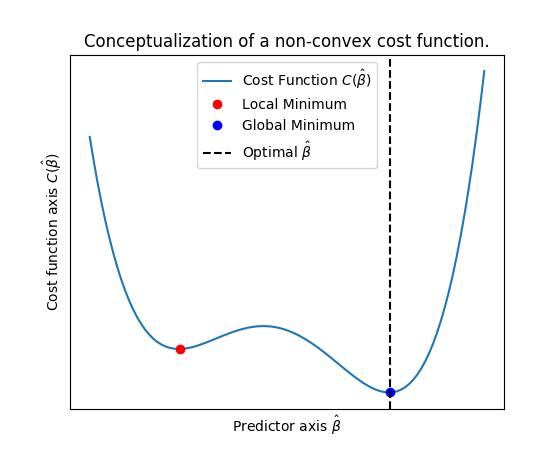
\includegraphics[width=0.4\textwidth]{figures/local_min_concept.png}
                \caption{Local minimum vs. Global minimum of non-convex cost function conceptualization figure.}
                \label{fig:local_min}
            \end{figure}
            There are a few practical solutions to solving the problem of local cost function minimum (such as using an adaptive learning rate to "anneal" closer to the global minimum \cite{stackexchangeminimum}), but the solution introduced in this research is using \textit{data batches}. This will be introduced briefly for the SGD solver, and described in further detail later on in the \textbf{Neural Network Dynamics} section.\\\\
            The SGD method is initialized with a guess $\hat{\beta}_0 \neq 0$, and the output $\sigma(\hat{y}_0=X\hat{\beta}_0)$ is calculated using the sigmoid function from equation \ref{eq:sigmoid}. This will typically be a poor guess, resulting in the error between the training data $y$ and first prediction $\hat{y}_0$ being relatively large. To improve this, the following gradient is applied to the predictor $\hat{\beta}$:
            \begin{equation}
                \hat{\beta}_1 = \hat{\beta}_0 - \eta \nabla_{\hat{\beta}_0}C,
            \end{equation}
            where $\nabla_{\hat{\beta}_0}C$ is the gradient of the cost function with respect to the first guess $\hat{\beta}_0$, and $\eta$ is the so-called \textit{learning rate}. This is referred to as one iteration of the method, where $C(\hat{\beta}_1) < C(\hat{\beta}_0)$ is guaranteed given that the learning rate is well adjusted. This learning rate $\eta$ is a subject which dictates how large the step size of the descent is, if the step is too large, then the cost function is not guaranteed to decrease after the iteration. There are many ways of modeling the learning rate, making this a central parameter of interest of the study presented. The learning rate will be discussed in greater detail later, though keep in mind that it is an adjustable parameter that is typically quite small, similar to the $l2$ regularization hyperparameter $\lambda$ (this will be presented later on).
            \\\\
            As previously mentioned, the $MSE$ cost function is used for linear regression, and the \textit{categorical cross-entropy} cost function is used for logistic regression
            %(classification) 
            cases. The categorical cross-entropy is found by taking the negative log of the so-called \textit{Maximum Likelihood Estimation}:
            \begin{align}
                \begin{split}
                    &P(\mathds{D}|\hat{\beta}) =\\ \prod^{n-1}_{i=0} \left[ p(y_i=1|x_i, \hat{\beta}) \right]^{y_i}&\left[ 1-p(y_i=1|x_i, \hat{\beta}) \right]^{1-y_i},
                \end{split}
            \end{align}
            which is defined as the total likelihood for all possible outcomes of a data set $\mathds{D}=\{ (x_i, y_i) \}$ which has binary labels $y_i \in \{ 0,1 \}$. Taking the negative logarithm of these probabilities produces the generalized categorical cross-entropy, or log-likelihood, cost function expression:
            \begin{align}
                \begin{split}
                    C(\hat{\beta}) &= \sum_{i=0}^{n-1} \bigg( y_i\log p(y_i=1|x_i, \hat{\beta}) \\&+ (1-y_i)\log\left[1-p(y_i=1|x_i, \hat{\beta})\right] \bigg),
                \end{split}
            \end{align}
            or rewritten as \cite{lecturenotes}:
            \begin{equation}
                C(\hat{\beta}) = -\sum^{n-1}_{i=0} \big( y_i \hat{y}_i - \log\left( 1 + \exp(\hat{y}) \right) \big).
            \end{equation}
            Applying the gradient of $\hat{\beta}$ to the cross-entropy function
            \begin{equation}
                \nabla_{\hat{\beta}}C =
                \begin{pmatrix}
                    \pdv{}{\hat{\beta}_0} \\
                    \pdv{}{\hat{\beta}_1} \\ 
                    \vdots \\ 
                    \pdv{}{\hat{\beta}_{p-1}} \\ 
                \end{pmatrix}C,
            \end{equation}
            where $\hat{\beta}_i$ is the $i$-th component of the vector (not to be confused with the iterations of the SGD algorithm), yields:
            \begin{equation}
                \nabla_{\hat{\beta}} C = -X^T\left( y - p \right),
            \end{equation}
            where $p=\sigma(\hat{y})$ is the prediction produced by $\hat{\beta}$. This is the gradient step introduced previously, yielding our expression for the stochastic gradient descent algorithm to be:
            \begin{equation}
                \hat{\beta}_{k+1} = \hat{\beta}_k - \eta \left( -X^T\left( y-\sigma(X\hat{\beta}_k) \right) \right).
            \end{equation}
            This is iterated until the gradient is so small that $\hat{\beta}_{k+1} \approx \hat{\beta}_k$, which is declared to be a sufficient predictor. This is the iterative gradient descent method used to minimize the categorical cross-entropy cost function, specifically for the sigmoid function $\sigma (\hat{y})$. See to M.H. Jensen's FYS-STK4155 Lecture notes for more detail on deriving these expressions \cite{lecturenotes} (Logistic Regression section of the citation).\\\\
            To avoid encountering any local minimum of the cost function, there is a random, or stochastic, factor included. This is known as the application of \textit{mini-batches}, where the gradient is split up into multiple 'sub-gradients':
            \begin{equation}
                \nabla_{\hat{\beta}} C = \sum^{B}_{b=1} \nabla_{\hat{\beta}_b} c,
            \end{equation}
            where $B$ is the number of batches and $b$ is a mini-batch. This concept of batches will be described in greater detail later on, when they are put into an ANN context.
    
    \subsection{Neural Network Dynamics}
        An ANN is generally a large system of many components which can be customized to conduct all kinds of studies. Before we can go into detial on the design of the network we will introduce the two most important algorithms to a neural network. These are the algorithms responsible for prediction and learning, the so-called \textit{Feed-Forward}, and \textit{Backwards-Propagation} algorithms, respectively.
        \subsubsection{Feed-Forward}
            The general theory of the neural network is to predict using the following linear equation:
            \begin{equation}\label{eq:z1}
                z = X W + b,
            \end{equation}
            where $X$ is the input data set, $W$ are the associated weights, and $b$ is the bias associated with the output. Figure \ref{fig:MLP_conc} illustrates the output of a single neuron:
            \begin{figure}[H]
                \centering
                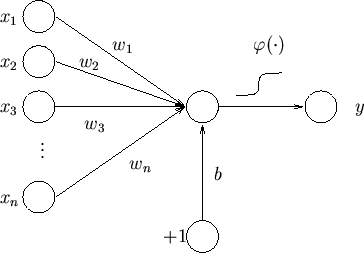
\includegraphics[width=0.4\textwidth]{figures/MLP.png}
                \caption{An illustration of how the inputs $X$ and weights $W$ and bias $b$ feed into a single neuron. Image taken from Antti Honkela.}
                \label{fig:MLP_conc}
            \end{figure}
            An \textit{activation function} is applied to $z$ to break the linearity of the equation, such that the output is transformed to:
            \begin{equation}\label{eq:a1}
                a = f\left( X W + b \right),
            \end{equation}
            where $f$ is the activation function. In figure \ref{fig:MLP_conc}, the symbol $\varphi$ represents the activation function. In this report, the function will be signified by $f$.\\\\
            It is worth noting that this is identical to the SGD system introduced in the previous section, where the predictor $\hat{\beta}$ is now replaced by the weights $W$, and the activation for the $SGD$ method was the sigmoid function $f=\sigma$. The difference is that the neural network is designed to have multiple \textit{layers} of such equations. Increasing the number of layers within the neural network is simple: The outputs of one layer become the inputs to the next layer, and so on. The extra/new layers are referred to as 'hidden'. Figure \ref{fig:MLP_full} illustrates what this looks like for three such layers (two of which are referred to as 'hidden'):
            \begin{figure}[H]
                \centering
                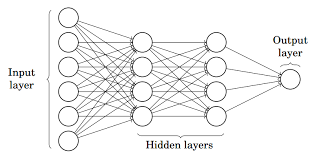
\includegraphics[width=0.4\textwidth]{figures/MLP2.png}
                \caption{A fully connected ANN illustration of two hidden layers and one output neuron. Image taken from: Vojtech Pavlovsky}
                \label{fig:MLP_full}
            \end{figure}
            Generalizing to a multilayer perceptron (MLP, simply means more than one layer) network yields the equations:
            \begin{align}
                a^1 &= f^1\left(X W^1 + b^1\right) \\
                a^2 &= f^2\left(a^1 W^2 + b^2\right) \\
                a^3 &= f^3\left(a^2 W^3 + b^3\right),
            \end{align}
            and so on, where $f^1$, $f^2$, and $f^3$ are activation functions (e.g. sigmoid), and $W^i$ and $b^i$ are the weights and biases corresponding to the output $i$. The general equations for the activation $a$ for a given layer $l$ are then given by:
            \begin{align}\label{eq:zWb}
                z^l &= a^{l-1}W^l + b^l\\\label{eq:afz}
                a^l &= f^l(z^l).
            \end{align}
            Here, $f^l$ is the activation function of layer $l$. It is good to keep these activation functions vague/general, as there are many such functions to choose between and the layers do not necessarily have the same ones.\\\\
            The \textit{feed forward} algorithm combines the weights and biases associated with the neural network to produce an output $\hat{y}$ in the following fashion:
            \begin{enumerate}
                \item Initialize by calculating $z^1$ and $a^1$ using equations \ref{eq:z1} and \ref{eq:a1}
                \item Save these and feed forward the activation from layer 1 to layer 2, calculating $z^2$ and $a^2$ using equations \ref{eq:zWb} and \ref{eq:afz} respectively.
                \item Continue this process until you get to the final output layer $l=L$, where $a^L=f^L(z^L)=\hat{y}$ is the prediction.
            \end{enumerate}
            Since we are operating on a set of data which has a binary output 1 (default) or 0 (not default), then the final activation function $f^L$ will always be the sigmoid function $\sigma$ (for the same reasons as presented in the SGD section). Further explanation of activation functions and their variants are presented later on.\\\\
            After the output $a^L=\hat{y}$ of the network is produced and all parameters $z^l$ and $a^l$ (for $l\in 1, 2, 3 \hdots L$) are calculated, then the backwards propagation algorithm can be initiated.
        
        \subsubsection{Backwards-Propagation}
            The backwards propagation algorithm is an essential step to the network \textit{learning} from its mistakes. The algorithm assesses the performance of the output $\hat{y}$, searches for the weights and biases which were most responsible for the inaccurate results, and tries to correct them to perform better. In essence this is a gradient descent algorithm, as the goal is once again to find a global cost function minimum:
            \begin{equation}
                \pdv{C}{\theta} = 0,
            \end{equation}
            where $\theta$ represents all the adjustable parameters of the regression. In the case of simple OLS, $\theta$ is the predictor $\hat{\beta}^{OLS}$, and in the case of the neural network, $\theta$ is the set of weights and biases $\theta \in (W, b)$. The backwards propagation algorithm aims to calculate the two parameters
            \begin{equation}
                \pdv{C}{W} \text{ and } \pdv{C}{b}
            \end{equation}
            in order to adjust the current weights $W$ and $b$ to decrease the cost function:
            \begin{equation}
                W = W - \pdv{C}{W} \text{ and } b = b - \pdv{C}{b}.
            \end{equation}
            This is done iteratively in the same fashion as the SGD algorithm.\\\\
            To derive expressions for these partial derivatives, the following chain rule trick is used:
            \begin{align}\label{eq:NNWdC/dW}
                \pdv{C}{W^l} &= \pdv{C}{z^l}\pdv{z^l}{W^l},\\\label{eq:NNWdC/db}
                \pdv{C}{b^l} &= \pdv{C}{z^l}\pdv{z^l}{b^l},
            \end{align}
            where $W^l$ and $b^l$ represent the weights and biases of layer $l$. The first component of layer $l=L$ needs to be calculated separately for the algorithm, before propagating backwards through layers $l \in [L-1, L-2, \hdots, 1]$. These following four partial derivatives are therefore all that is needed to perform back propagation:
            \begin{equation}\label{eq:bp_pdvs}
                \pdv{C}{z^L} \text{, } \pdv{C}{z^l} \text{, } \pdv{z^l}{W^l} \text{, and } \pdv{z^l}{b^l}.
            \end{equation}
            In this paper, the partial derivative of the cost function with respect to the weighted output $z^l$ will often times be referred to as:
            \begin{equation}
                \delta^l = \pdv{C}{z^l}.
            \end{equation}
            To derive expressions for the four essential partial derivatives presented in equation \ref{eq:bp_pdvs}, the final layer $l=L$ is first examined. Another chain rule trick yields:
            \begin{equation}
                \pdv{C}{z^L} = \pdv{C}{a^L} \pdv{a^L}{z^L},
            \end{equation}
            and utilizing the relation between $a$ and $z$ presented in equation \ref{eq:afz} yields the following:
            \begin{equation}
                \pdv{C}{z^L} = \nabla_a C \odot f'^L(z^L).
            \end{equation}
            This is one of our equations, and is kept general for the sake of cost- and activation function flexibility. $\nabla_aC$ represents the gradient of $C$ with respect to the output $a^L$, $f'^L$ is the derivative of the activation function of the output layer, and the $\odot$ operator represents element-wise multiplication. This is also known as the Hadamard product. Moving on to the next equations, we use another chain rule trick:
            \begin{align}\label{eq:C/zl}
                \pdv{C}{z^l} &= \pdv{C}{z^{l+1}} \pdv{z^{l+1}}{a^l} \pdv{a^l}{z^l}.\\
                \delta^l &= \delta^{l+1} \pdv{z^{l+1}}{a^l} \pdv{a^l}{z^l}.
            \end{align}
            This product consists of elements which we can express differently, namely as:
            \begin{align}\label{eq:C/zl1}
                \pdv{z^{l+1}}{a^l} &= \pdv{}{a^l}\left( a^lW^{l+1} + b^{l+1} \right)=W^{l+1}\text{, and}\\\label{eq:C/zl2}
                \pdv{a^l}{z^l} &= f'^l(z^l).
            \end{align}
            Inserting equations \ref{eq:C/zl1} and \ref{eq:C/zl2} into equation \ref{eq:C/zl} leaves us with the following expression:
            \begin{align}
                \pdv{C}{z^l} &= \left( (W^{l+1})^T \pdv{C}{z^{l+1}}  \right) \odot f'^l(z^l)\\
                \delta^l &= \left( (W^{l+1})^T \delta^{l+1}  \right) \odot f'^l(z^l)
            \end{align}
            This is another one of the equations required for the backwards propagation algorithm. Now, examination of the final terms yields:
            \begin{align}
                \pdv{z^l}{W^l} &= \pdv{}{W^l}\left( a^{l-1}W^l + b^l \right) = a^{l-1}\\
                \pdv{z^l}{b^l} &= \pdv{}{b^l}\left( a^{l-1}W^l + b^l \right) = 1.
            \end{align}
            Inserting all these relations back into equations \ref{eq:NNWdC/dW} and \ref{eq:NNWdC/db} yields:
            \begin{align}
                \pdv{C}{b^l} &= \delta^l \ \text{,  and}\\
                \pdv{C}{W^l} &= (a^{l-1})^T\delta^l.
            \end{align}
            The four equations for the backwards propagation algorithm can then be summarized by rewriting the vectors with index notation:
            \begin{align}
                \delta^L &= \nabla_a C \odot f'^L(z^L), \\
                \delta^l &= ((W^{l+1})^T\delta^{l+1})\odot f'^l(z^l), \\
                \pdv{C}{b^l_j} &= \delta^l_j, \\
                \pdv{C}{W^l_{j,k}} &= a^{l-1}_k\delta^l_j,
            \end{align}
            where $\nabla_aC$ is the gradient of the cost function w.r.t. the output $a$, and $f'^l$ is the derivative of the activation function of layer $l$ w.r.t. $z^l$. \\\\
            This is all that is needed to ensure that the weights and biases can be corrected in a manner that reduces the cost function $C$ in relation to the adjustable parameters $\theta \in \left(W,b\right)$. Once again, there is the possibility of being caught in a local minimum in the case of a non-convex cost function $C$. The learning rate $\eta$ and batch concepts are therefore presented in the ANN context, though they are very similar to what was presented for the SGD section.
            
        \subsubsection{Learning rate, batches and $l2$ regularization}
            To research the impact of these gradient factors to the biases and weights, a learning rate is included to control the size of the steps. This is identical to the SGD learning rate $\eta$, which is simply a value which the gradients are multiplied with. The backwards propagation algorithm now updates the biases and weights by the factors:
            \begin{align}
                b^l_j &= b^l_j - \eta \pdv{C}{b^l_j}, \\
                W^l_{j,k} &= W^l_{j,k} - \eta \pdv{C}{W^l_{j,k}}.
            \end{align}
            There are several ways of modeling the learning rate, some of which involves the \textit{adaptive} learning rate or the \textit{time-based} learning rate. However, these are not implemented into the current research. The learning rate will be set to a typically small constant value throughout the project. The best learning rate value is a topic which will be of interest when a search of the ANN which produces the most accurate predictions is researched.\\\\
            The neural network gradient is segmented into batches in a similar way to what was done in the SGD section. This is done to avoid the problem of local minimum of the cost function; a problem which has been introduced already. This is once again done by averaging the gradients of multiple inputs at a time, making it so that the input matrix $X$ is now of size $(batchsize \times p)$, and the weights and biases are now updated using the sum of these average gradients. The data set must be shuffled after each batch is iterated over using the feed-forward and backwards propagation algorithms presented. This is done to further increase the likelihood of the algorithm to reach a global minimum, as the averages will differ slightly depending on the batchsize. If the batchsize is large, then the average of the batch gradient will typically not change very drastically; the batchsize is therefore recommended to be around $B=100$. This is already quite a large number of cases, so should not be increased much more. After each of the batches have updated the weights and bias gradients and the data set is shuffled, a new \textit{epoch} begins. This signifies all the data has been cycled through and the gradients have been updated accordingly. This equates to one 'iteration' $k\rightarrow k+1$ of the SGD method presented previously. The number of epochs is not quite as important as the change in the gradients $per$ epoch. As, if an epoch does not cause the weights and biases to change very much, then the current parameters are declared as sufficient to produce a cost function minimum.\\\\
            One more subject is introduced before moving onto an introduction of cost- and activation functions, namely l2 regularization. The learning rate is one of the parameters which is adjustable and of interest, the other one being the l2 regularization hyperparameter $\lambda$. The l2 regularization involves adding an additional factor/penalty to the original cost function $C_0$, such that:
            \begin{equation}
                C = C_0 + \frac{\lambda}{2n} \sum_j |W_j|^2
            \end{equation}
            is the new cost function, where $p$ is the number of features. This ultimately penalizes the weights if they are too large, making it so that the weights $W$ are encouraged to be smaller. The net impact of this factor is that the derivative of the cost function w.r.t. the weights presented earlier now has an additional factor which subtracts a fraction of the current weights:
            \begin{align}
                W^l_{j,k} &= W^l_{j,k} - \eta\left[ \pdv{C_0}{W^l_{j,k}} + \frac{\lambda}{n} W^l_{j,k} \right]\\
                W^l_{j,k} &= \left(1-\frac{\eta\lambda}{n}\right)W^l_{j,k} - \eta \pdv{C_0}{W^l_{j,k}},
            \end{align}
            where $\eta$ is the learning rate, $\lambda$ is the $l2$ regularization hyperparameter, $C_0$ is the cost function without $l2$ regularization, and $p$ is the number of features/inputs into the network. This hyperparameter $\lambda$ is something which will be studied in detail in an attempt to find the value which produces the most accurate $\hat{y}$ prediction.
            
    \subsection{Cost- and Activation functions}
        A quintessential component to the neural network system is the choice of cost- and activation functions. The feed-forward system is dictated and fed through multiple activation functions, vastly influencing the outcome. This will be a large point of debate in the methods, results and the discussion section. A few cost- and activation functions will be presented here for this study, though far more variants exist in their respectful families. Table \ref{tab:cost_functions} lists a few cost functions which are explored, and their respectful derivatives:
        \begin{table}[H]
            \centering
            \begin{tabular}[t]{l@{\hskip 0.1in}c@{\hskip 0.1in}c}
                \toprule
                 & $C(y, a^L)$ & $\nabla_aC(y, a^L)$\\
                \midrule
                 &  & \\
                Mean-Squared Error & $\mathds{E} \left[ \frac12 (y-a^L)^2\right]$ & $a^L-y$ \\ & & \\
                Cross-Entropy & $\begin{cases}-\log(a^L) & \text{if } y=1\\ -\log(1-a^L) & \text{if } y=0\end{cases}$ & $a^L-y$ \\ & & \\
                \bottomrule
            \end{tabular}
            \caption{Several cost function examples. Mainly, the cross-entropy and mean-squared error (MSE) functions will be explored in this study. As explained previously, the activations of the final layer $a^L$ are equivalent with the prediction of $y$, namely $\hat{y}$. }
            \label{tab:cost_functions}
        \end{table}
        The symbol $\mathds{E}$ indicates the \textit{expectation value} of some list of values, formally defined as:
        \begin{equation}
            \mathds{E}\left[a\right] = \sum_{i=0}^{n-1} a_i \cdot P(a_i),
        \end{equation}
        where $P(a_i)$ is the probability of the outcome $a_i$. When the results are uniformly distributed, or have equal outcomes, then the expectation value is given by
        \begin{equation}
            \mathds{E}\left[a\right] = \frac1n\sum_{i=0}^{n-1} a_i.
        \end{equation}
        \subsubsection{Mean-Squared Error}
            Mean-squared error, or the \textit{L2 loss function} is the most typical cost function to use in non-logistic regression cases. This is a very consistent and simple function to measure the performance of a prediction $\hat{y}$ in relation to the training data $y$.
        \subsubsection{Cross-Entropy}
            The most common cost function used in logistic regression is the cross entropy, or \textit{log-loss} function. The function listed in the table measures the performance of a classification model, where all outputs are set to be between 0 and 1. This function stems from the \textit{Maximum Likelihood Estimation} principle presented previously.
            This cross entropy expression is specific to the case of binary classification. 
            This is the case for the credit card data logistic regression, so the cross-entropy is the cost function of choice for neural network logistic regression study. \\\\
	        These are the two choice cost functions to perform the classification and regression research. In addition to choosing a cost function for predicting, one must also make a choice of activation functions. Table \ref{tab:activation_functions} lists a few activation functions which are explored, and their respectful derivatives:
	        \begin{table}[H]
	            \centering
	            \begin{tabular}[t]{l@{\hskip 0.4in}c@{\hskip 0.3in}c}
	                \toprule
	                 & $f(z_i)$ & $f'(z_i)$ \\
	                \midrule\\
	                Sigmoid & $(1+e^{-z_i})^{-1}$ & $f(z_i)\left( 1-f(z_i) \right)$ \\\\
	                tanh & $\tanh (z_i)$ & $1-f^2(z_i)$ \\\\
	                ReLU & $\begin{cases} z_i & \text{for } z_i>0 \\ 0 & \text{else} \end{cases}$ & $\begin{cases} 1 & \text{for } z_i>0 \\ 0 & \text{else} \end{cases}$ \\\\
	                ReLU6 & $\begin{cases} z_i & \text{for } z_i\in[0,6] \\ 0 & \text{for } z_i<0 \\ 6 & \text{for } z_i>6 \end{cases}$ & $\begin{cases} 1 & \text{for } z_i\in [0,6] \\ 0 & \text{else} \end{cases}$ \\\\
	                Softmax & $e^{z_i}\cdot(\sum_k e^{z_k})^{-1}$ & $\begin{cases}s_i(1-s_j) & \text{for } i=j\\ -s_i\cdot s_j & \text{for } i\neq j \end{cases}$ \\\\
	                Softsign & $z_i\cdot \left( 1+|z_i| \right)^{-1}$ & $\left( 1+|z_i| \right)^{-2}$\\\\
	                \bottomrule
	            \end{tabular}
	            \caption{Table listing a number of common activation functions and their derivatives. Several of these are of interest and are implemented into the study.}
	            \label{tab:activation_functions}
	        \end{table}
	        These are some key activation functions which may be studied. One thing to note is that the derivative of the softmax function is a matrix since the activation of node $a_j$ can depend on all the other activations from the denominator $\sum_ke^{z_k}$ of the function. Technically, the derivative stated in the table is really the derivative $\pdv{}{a_j}f(z_i)$. Following is a short discussion of the strengths and some weaknesses of some of the activation functions introduced in table \ref{tab:activation_functions}:
        \subsubsection{Sigmoid function}
            The Sigmoid function is typical for predictive applications as it is bounded to $\sigma \in [0,1]$. This is useful for logistic regression purposes as discussed previously, though it does not come without its flaws. The sigmoid function has the problem of \textit{vanishing gradients} for values outside of the range (approximately) $x \in [-6,6]$. The derivative of the sigmoid is consistently vanishing in these areas $\sigma'(z)\approx 0$ for $z\in [\leftarrow, -6]\vee[6, \rightarrow]$, resulting in the weights and biases not being updated properly in the backwards propagation algorithm. This problem can however be circumvented through proper data preprocessing and weights initialization. If the node values $z$ values are within this range, the network should be able to tell the difference between them in the gradient. This requires the inputs $X$ to be scaled correctly as well as the weights and biases to not be too large.
        \subsubsection{Tanh function}
            Although the hyperbolic tangent function has different bounds than the sigmoid function, ranging from $-1$ to $1$, it can just as easily be applied to binary classification cases. The only difference needed is to edit th training and testing data to have the same ranges. In the case of the binary credit card classification, all the zeros would need to be changed to $-1$'s. This is not done in this study, though it is a possibility. This function also has vanishing gradients for large values, though this can be avoided by proper data processing once again. 
        \subsubsection{ReLU6}
            ReLU is shown to be specifically good for image recognition applications \cite{ReLUImagenet}. Keeping to the same family, though introducing an upper bound of $6$ is useful in this case. ReLU6 is therefore an excellent variant of the ReLU function, keeping some of it's characteristics and making sure that it is bounded from both below and above.
        \subsubsection{Weight- and Bias Initialization}
            Xavier and He \cite{He2015} conducted researched regarding what the best bias and weight initialization expressions were, and found that the following are the optimal mean- and standard deviation values for the weights (specifically for the ReLU activation function family):
            \begin{equation}\label{eq:xavier}
                \mu = 0 \text{ and } \sigma = \sqrt{\frac{2}{n_i+n_{i+1}}},
            \end{equation}
            where $n_i$ is the number of nodes in the current layer, and $n_{i+1}$ is the number of nodes in the next layer. The weights are initialized randomly with these parameters, and the biases are initialized as zero in this scheme, henceforth referred to as the \textit{Xavier initialization}.\\\\
            Other initialization schemes can come up, though it is very important that these are not large in absolute value. This may cause vanishing gradients in some of the activation functions, as mentioned above. 
        
    \subsection{Classification}
        
        % GOAL: use two different methods NN and LR and compare the two: which has best accuracy?
            % Present logistic regression and neural networks as the two methods that we will use
            % Introduce the cost function which will be used for LR and NN (MSE and cross entropy)
            % Introduce accuracy score
            % Present regularization parameters and learning rates
        
        
        % Present LR as a general classification method
        % Introduce our choice of LR: SGD with mini-batches
    
        
    
        % INSPO
        % 2.1.2. Logistic regression (LR) Logistic regression can be considered a special case of linear regression models. However, the binary response variable violates normality assumptions of general regression models. A logistic regression model specifies that an appropriate function of the fitted probability of the event is a linear function of the observed values of the available explanatory variables.  
        % ---- The  major  advantage  of  this approach is that it can produce a simple probabilistic formula of classification. 
        % ---- The weaknesses are that LR cannot properly deal with the problems of non-linear and interactive effects of explanatory variables.
        
        \subsubsection{Neural Network Application}
            The neural network applied to the classification data is what is known as a \textit{multilayer perceptron}. This means that the network consists of non-linear activation functions and a scheme of fully-connected weights and biases. Also, each of the neurons from layer $i$ are connected by a weight and a bias to the neurons in layer $i+1$ and so on.
        % Present what a NN is and how it is set up
        % Present our NN: which is feed forward neural network by using back propagation
        % Introduce weights, biases, regularization parameters and learning rates
        % Activation function: tanh (hyperbolic tangent), sigmoid (the logistic function, ReLU (overcome numerical problems related to the sigmoids)
        % Fully connected FFNN (each node is connected to all nodes in previous layer)
      
      
        % INSPO
        % 2.1.5. Artificial neural networks (ANNs)Artificial neural networks use non-linear mathematicalequations to successively develop meaningful relationships between input and output variables through a learning pro-cess. We applied back propagation networks to classify data. A back propagation neural network uses a feed-for-ward topology and supervised learning. The structure of back propagation networks is typically composed of aninput layer, one or more hidden layers, and an outputlayer, each consisting of several neurons. ANNs can easilyhandle the non-linear and interactive effects of explanatoryvariables. The major drawback of ANNs is – they cannotresult in a simple probabilistic formula of classification
        % WHY multilayer perceptrons (Lectrue notes NN) According to the Universal approximation theorem, a feed-forward neural network with just a single hidden layer containing a finite number of neurons can approximate a continuous multidimensional function to arbitrary accuracy, assuming the activation function for the hidden layer is a non-constant, bounded and monotonically-increasing continuous function.
        \subsubsection{Accuracy Assertion of Classification}
            There are several ways to assert the accuracy of the logistic model. One which is the simplest and most intuitive is the \textit{accuracy score}, which measures the fraction of correctly guessed targets:
            \begin{equation}
                Acc = \frac1n\sum^{n-1}_{i=0} \mathds{1}(\hat{y}_i=y_i),
            \end{equation}
            where 
            \begin{equation}
                \mathds{1}(\hat{y}_i=y_i) = \begin{cases}1 & \text{if  }\ \hat{y}_i=y_i \\ 0 & \text{else}\end{cases}.
            \end{equation}
            This is the simplest accuracy metric possible, though there are some weaknesses to designing a model around maximizing this. A few more accuracy metrics are therefore introduced in this section for a more in-depth analysis of the performance of the classification methods. One of these is the so-called \textit{confusion matrix}:
            \begin{table}[H]
                \centering
                \begin{tabular}{cc|@{\hskip 0.1in}cc}
                     & & \multicolumn{2}{c}{True}\\
                     & & 0 & 1\\\hline & & & \\
                    \multirow{ 2}{*}{Pred} & 0 & TN & FP \\
                     & 1 & FN & TP
                \end{tabular}
            \end{table}
            This matrix conveys the model performance in greater detail than the accuracy score, as the errors FN and FP are \textit{not equivalent}. They are called \textit{false positives} and \textit{false negatives}, respectively. If the data being predicted is something like patient data rather than credit card data and the logistic regression involves predicting whether or not a patient has a malicious disease, then it is easier to imagine how these two differ. It is far worse to mis-classify a sick patient than a healthy one. In our case, if $1=$ sick, then we would like for FN to be as small as possible, but it is far more important that FP$\rightarrow 0$. Ultimately though, in any case, the perfect model diagonalizes this matrix, such that FP=FN=0. \\\\
            Two more accuracy metrics are the areas under the Cumulative Gain (CG) chart and the Receiver Operating Characteristics (ROC) curve. These two curves visualize the performance of the model in two different ways. Both curves have upper and lower boundaries, such that the relative areas under these curves are very useful to assess the results. Figures \ref{fig:conceptual_cumulative_gains} and \ref{fig:conceptual_ROC} illustrate the difference between these two curve shapes:
            \begin{figure}[H]
            	\centering
            	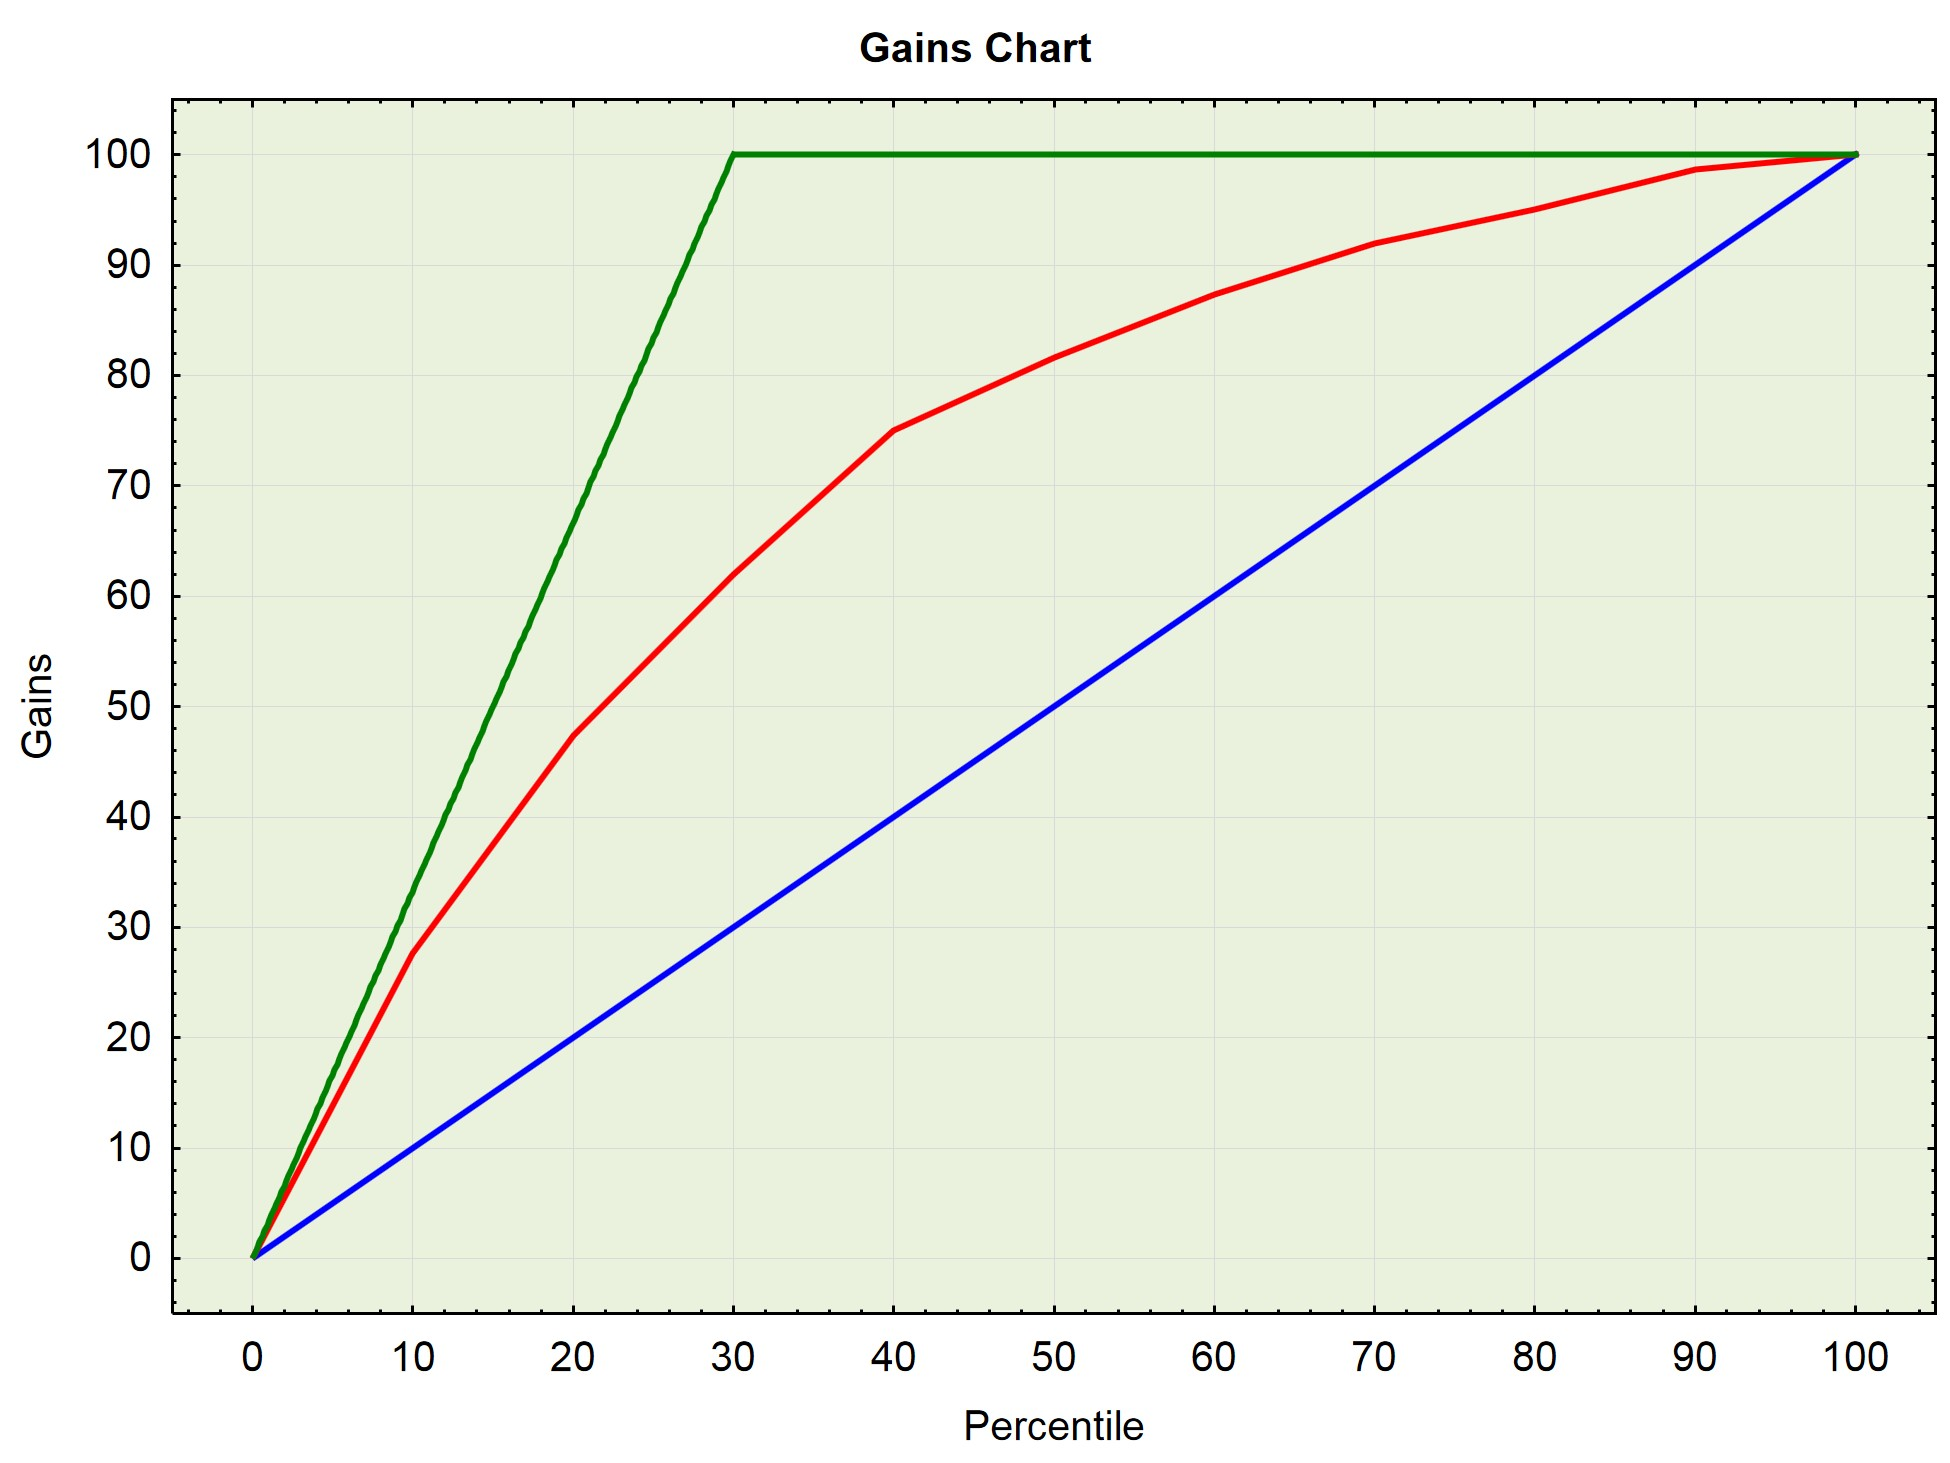
\includegraphics[width=0.4\textwidth]{figures/gains_chart.jpg}
            	\caption{Conceptualized figure of a cumulative gain chart. The figure includes perfect $100\%$ accuracy model, and a baseline illustrating what a random $50\%$ guess looks like. Image taken from Tomáš Jurczyk.}
            	\label{fig:conceptual_cumulative_gains}
            \end{figure}
	        \begin{figure}[H]
	        	\centering
	        	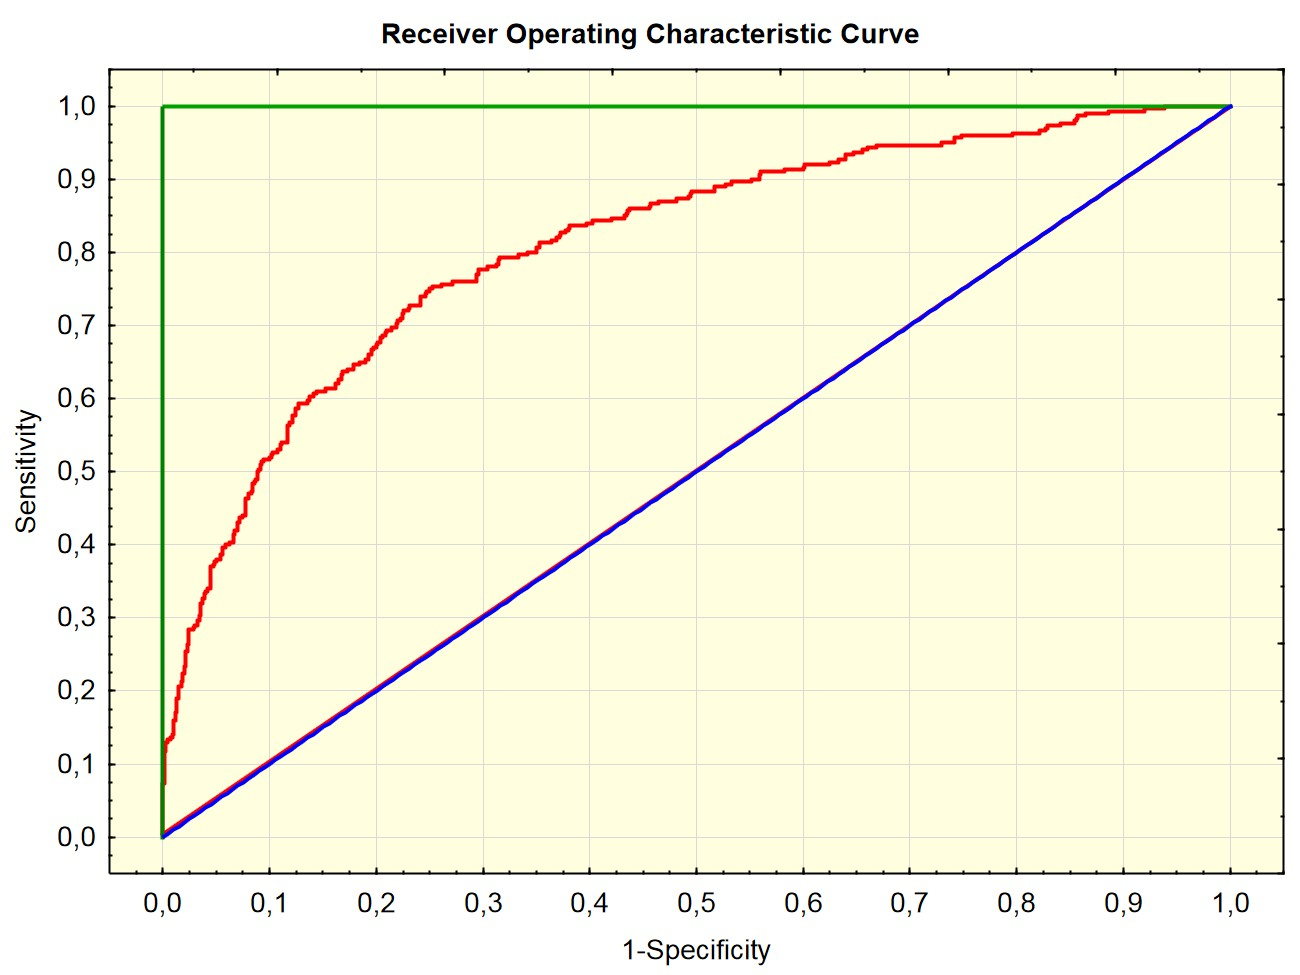
\includegraphics[width=0.4\textwidth]{figures/ROC.jpg}
	        	\caption{Conceptualized figure of the ROC curve. This figure also includes perfect $100\%$ accuracy model, and a baseline illustrating what a random $50\%$ guess looks like. Image taken from Tomáš Jurczyk}
	        	\label{fig:conceptual_ROC}
	        \end{figure}
        	These two figures look similar though they are not quite the same. The difference between the two prediction curves is the scale of the x-axis of the graphs. Both the CG chart and the ROC curve measure the same quantity in the y-axis, namely the \textit{Sensitivity} (otherwise referred to as the gains), which is given by the following expression:
        	\begin{equation}\label{eq:sensitivity}
        		\text{Sensitivity} = \frac{\text{TP}}{\text{TP} + \text{FN}},
        	\end{equation}
        	where TP is the count of the true positives and FN is the count of the false negatives. The primary distinction of the two curves is in the measurement made on the x-axis. The CG chart measures the following on the x-axis:
        	\begin{equation}
        		\frac{\text{TP} + \text{FP}}{\text{TN} + \text{FP} + \text{FN} + \text{TP}},
        	\end{equation}
        	where the denominator simply is the measure of the number of all observations. The ROC curve has an x-axis given by the following expression \cite{6}:
        	\begin{equation}
        		\frac{\text{FP}}{\text{TN} + \text{FP}}.
        	\end{equation}\\
            One more metric is finally introduced for binary classification assessment: The $F1$ Score. This is formally defined as
            \begin{equation}
                F_1 = 2\left(\frac{\text{Sensitivity}\cdot \text{Recall}}{\text{Sensitivity} + \text{Recall}}\right),
            \end{equation}
            where the Sensitivity is as defined in equation \ref{eq:sensitivity}, and the Recall (otherwise known as the True Positive Rate) is given by:
            \begin{equation}
                \text{Recall} = \frac{\text{TP}}{\text{TP}+\text{FP}}.
            \end{equation}
            The Sensitivity assesses the \textit{true positives} \text{TP} in relation to the \textit{false negatives} FN, while the Recall assesses the true positives in relation to the \textit{false positives} FP\cite{2}.
            
    \subsection{Regression}
        % GOAL: use NN and LR (linear regression) to fit Franke function data set
            % Present lin.reg and NN as the two methods for this problem
            % Present minimization of MSE (which will be used to compare the results)
        The goal with the regression study portion of the project is to use neural networks and linear regression methods to fit \textit{Franke's Function}. This function is typical to use when testing regression methods, and is given by:
        \begin{align}\label{eq:frankes_function}
            \begin{split}
                f(x, y) &= \frac{3}{4}\text{exp}\left(-\frac{(9x - 2)^2}{4} - \frac{(9y - 2)^2}{4}\right) \\
                &+ \frac{3}{4}\text{exp}\left(-\frac{(9x + 1)^2}{49} - \frac{(9y + 1)}{10}\right) \\
                &+ \frac{1}{2}\text{exp}\left(-\frac{(9x - 7)^2}{4} - \frac{(9y - 3)^2}{4}\right) \\
                &- \frac{1}{5}\text{exp}\left(-(9x - 4)^2 - (9y - 7)^2\right),
            \end{split}
        \end{align}
        This function exhibits a very interesting surface plot which is very recognizable in prediction data. The function surface is illustrated in figure \ref{fig:frankesfunction}
        \begin{figure}[H]
        	\centering
        	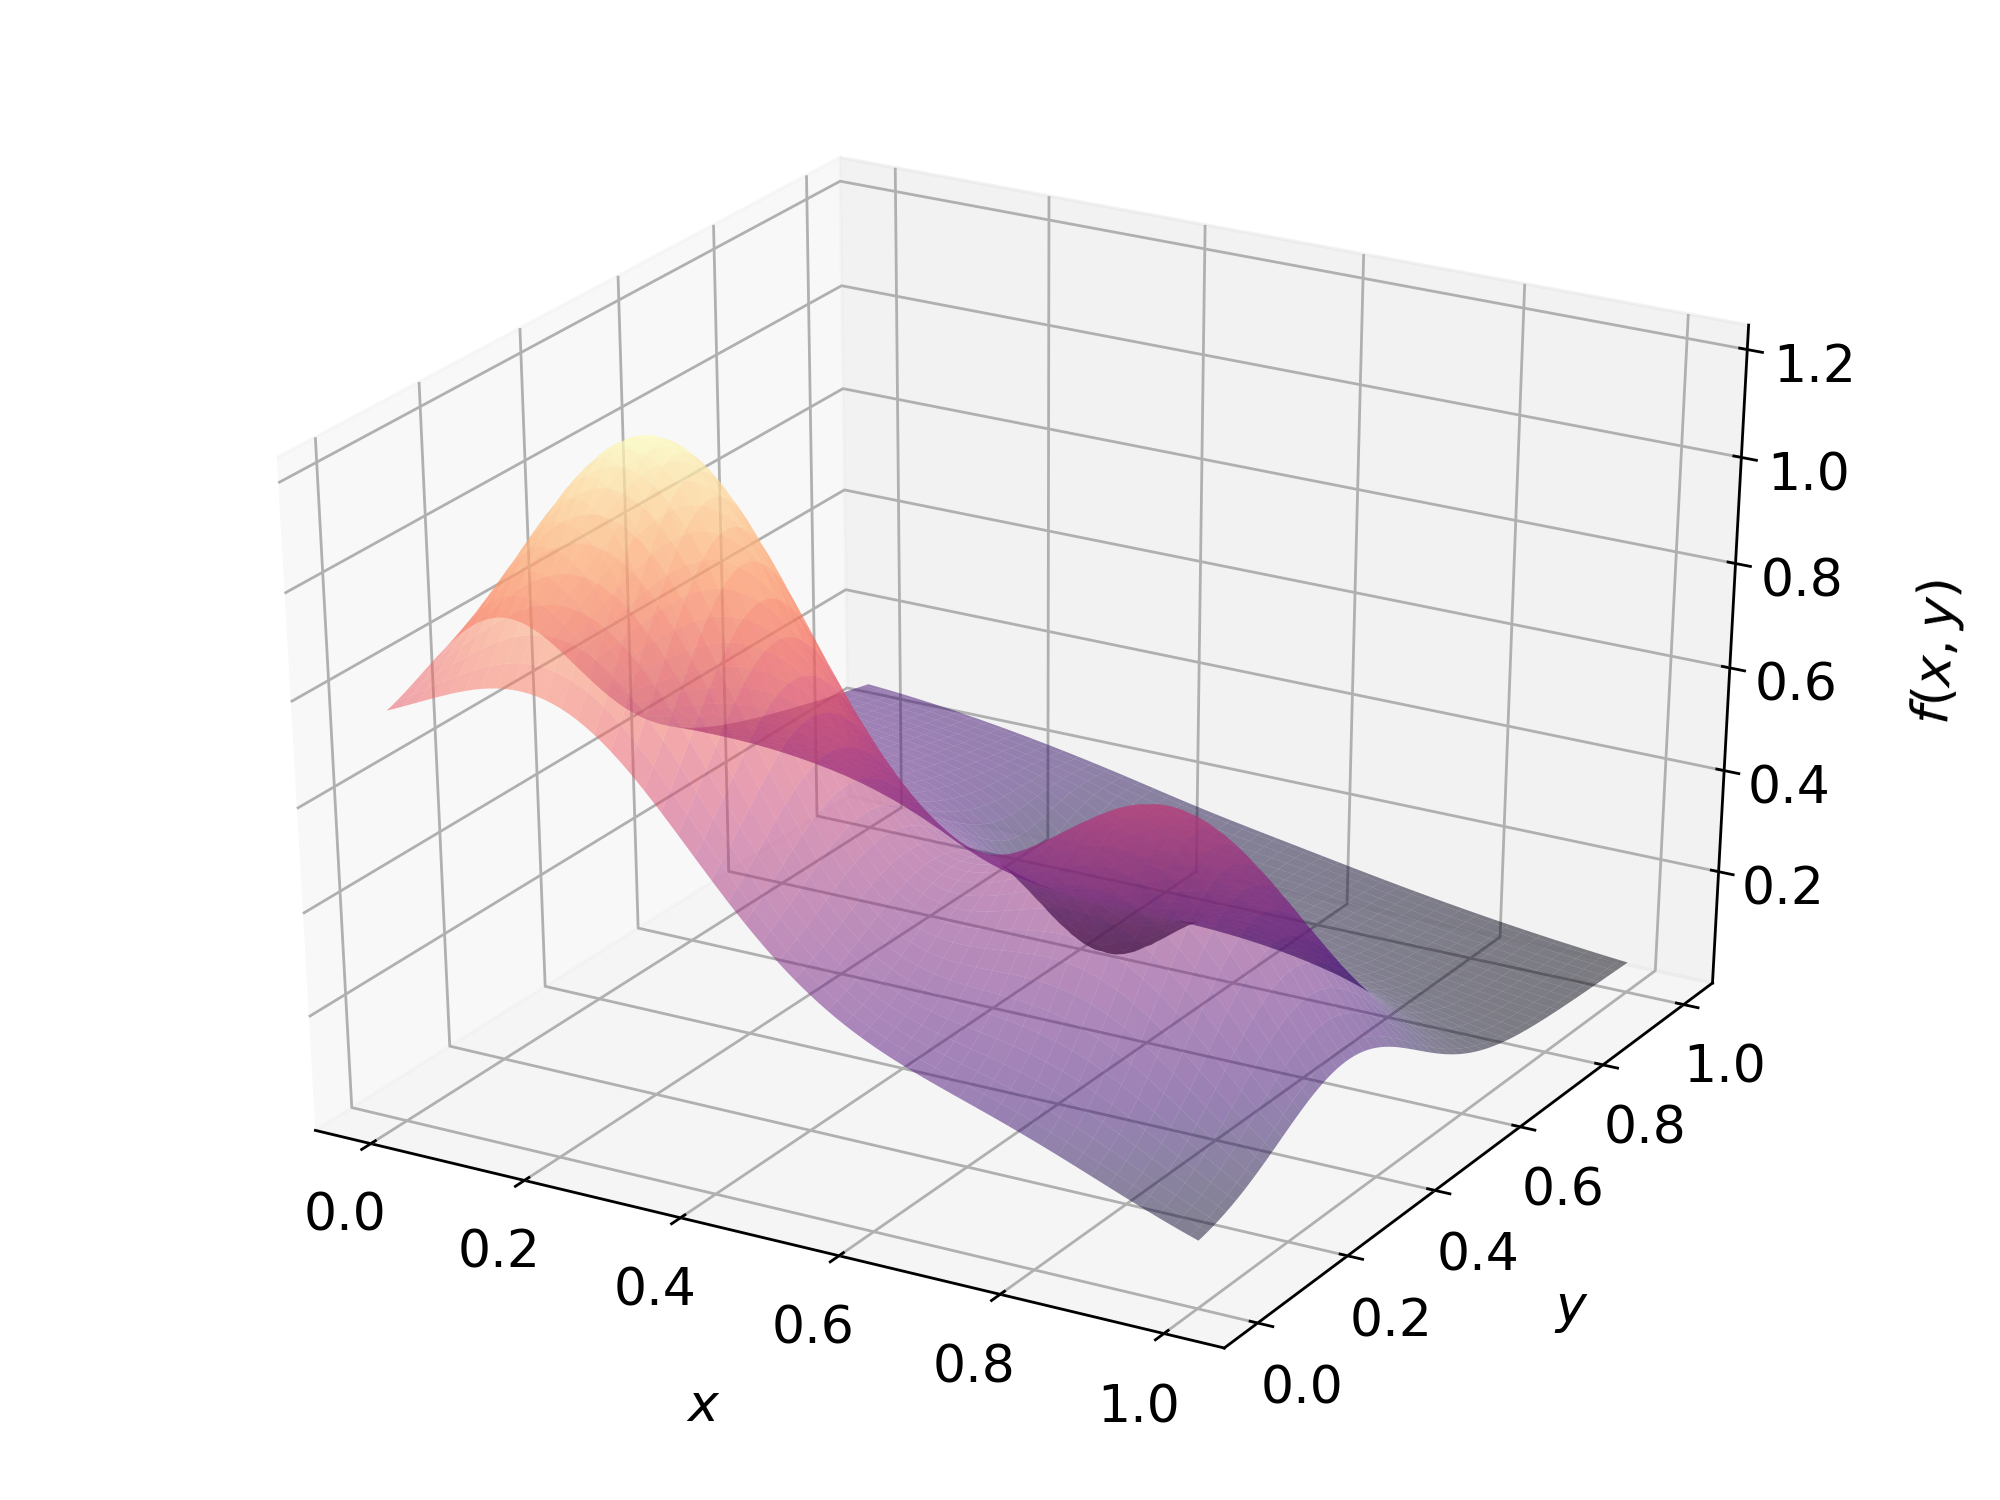
\includegraphics[width = 0.4\textwidth]{figures/Franke.png}
        	\caption{The \textit{Franke function} surface plot illustration for $x$ and $y$ values ranging from zero to one.}
        	\label{fig:frankesfunction}
        \end{figure}
       	Attempting to recreate this function using ridge regression and a neural network would be improper without some functional noise. Adding some noise (as a Gaussian distribution with $\mu=0$ and $\sigma=0.01$) produces the following data set:
        \begin{figure}[H]
        	\centering
        	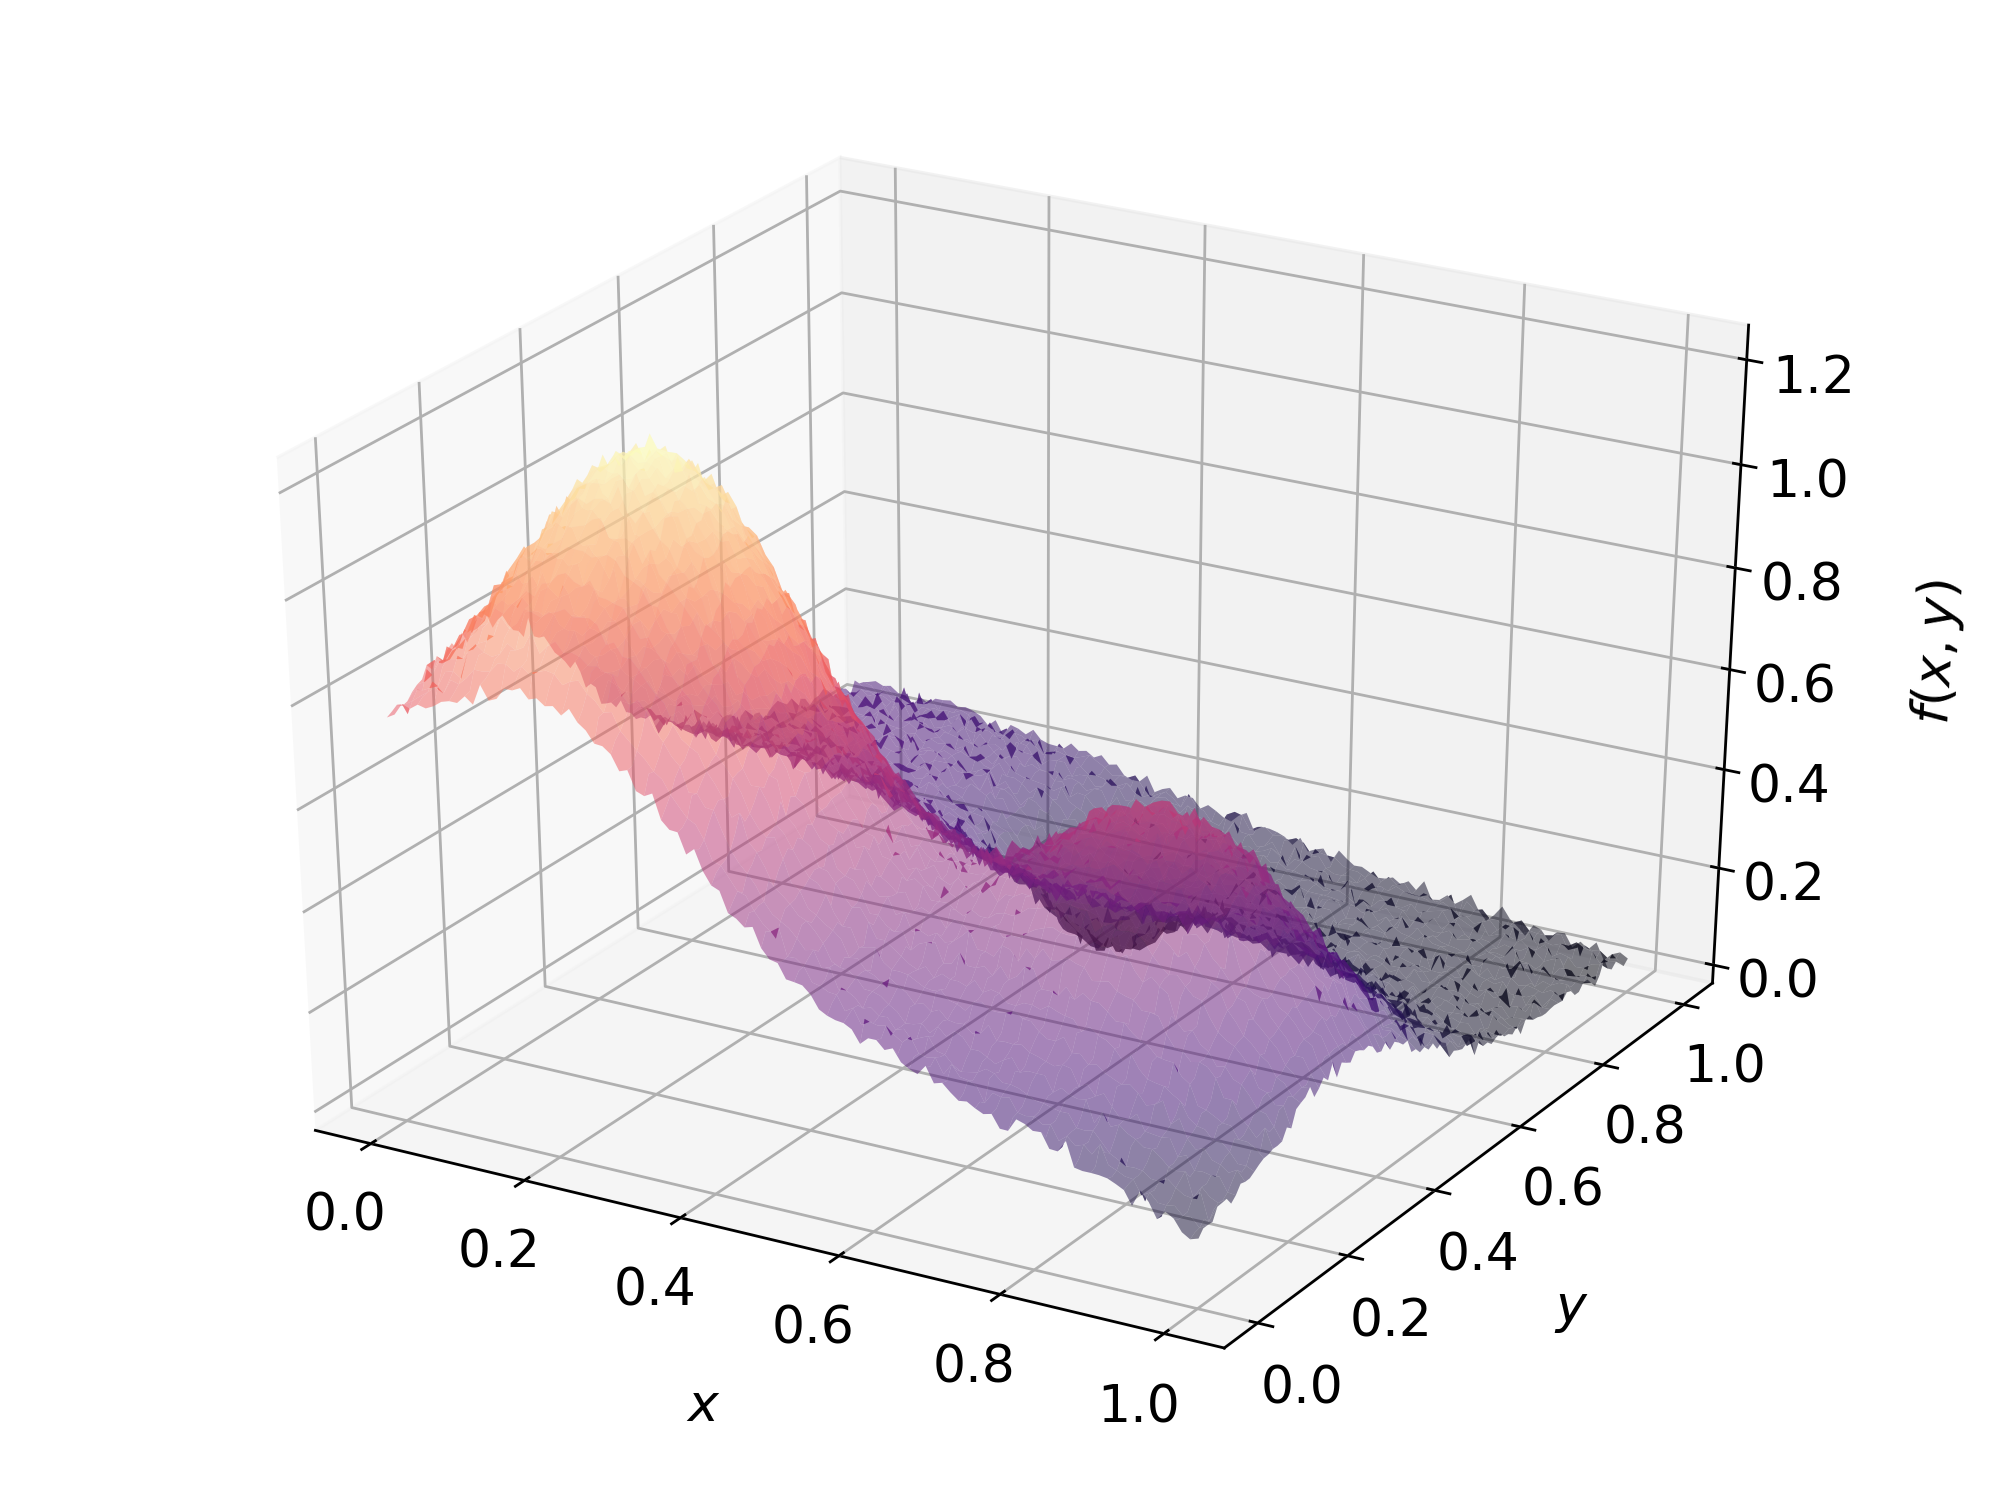
\includegraphics[width = 0.4\textwidth]{figures/Franke_noise.png}
        	\caption{The \textit{Franke function} surface plot illustration for $x$ and $y$ values ranging from zero to one. Random Gaussian noise with mean value $\mu=0$ and standard deviation $\sigma=0.01$ is added to each data point $f(x_i,y_i)$.}
        	\label{fig:frankesfunction}
        \end{figure}
        This is more similar to the data the methods will attempt to recreate. Two methods are implemented to attempt to reproduce Franke's function: \textit{Ridge Regression} %(presented previously) 
        and a \textit{Neural Network}, this time applied to data which is not classification-oriented.
        \subsubsection{Neural Network Application}
            % Cost function for regression case: RSS?
            % Best fit a surface by adjusting regularization parameters (RP) and learning rates: minimize MSE
            The neural network applied to the regression data is very similar to the classification network described previously. %(multilayer perceptron). 
            Now however, instead of a constant binary output $a^L\in[0,1]$, the network is trained to output the results of Franke's function. This means that the output activation function cannot be a function which bounded asymptotically; some common activation functions such as the \textit{Leaky ReLU} come to mind, though the most intuitive one is simply using the \textit{identity} $f(x)=x$. The research conducted on Franke's function will include the learning rate and hyperparameter as previously, so a search for an optimal value for both of these will once again be performed.
        \subsubsection{Accuracy Assertion of Regression}
        	% MSE for regression and R2 score. Introduce these.
        	The accuracy metrics used for the prediction of Franke's function are the MSE,%(introduced earlier)
        	and the so-called R2-Score. These two accuracy metrics are given by the following expressions:
        	\begin{align}
        		MSE(y, \hat{y}) &= \frac{1}{2n}\sum_{n-1}^{i=0} \left(y-\hat{y}\right)\\
        		R2(y, \hat{y}) &= 1 - \frac{RSS}{TSS},
        	\end{align}
        	where $RSS$ is the \textit{residual sum of squares}, and $TSS$ is the \textit{total sum of squares}. These are respectively defined as:
        	\begin{align}
        		RSS(y, \hat{y}) &= \sum^{n-1}_{i=0} \left(y-\hat{y}\right)^2\\
        		RSS(y, \hat{y}) &= \sum^{n-1}_{i=0} \left(y-\bar{y}\right)^2\\
        		\bar{y} &= \frac{1}{n}\sum^{n-1}_{i=0}y_i. 
        	\end{align}
        	These expressions are all that is needed to calculate the R2 score and MSE. As discussed earlier, we would like the MSE %(cost function in the case of regression) 
        	to be as small as possible. The R2 score is different, it is a score which is always in the domain of $R2\in [0,1]$, where $R2\rightarrow 1$ for a 'perfect model', meaning that the R2 score is a parameter we would like to maximize.
	
	\section{Method}
    The algorithms presented are implemented and simulated in Python3.6 using several libraries. Some of these have functions which are implemented explicitly; the PCA is for example implemented using a package from the scikit-learn library. This will be gone into further detail later on. Before building the neural network, the data must be prepared. This is called preprocessing.
    \subsection{Preprocessing of the Data Set}
        The most important section of any data analysis is getting to know and performing a preprocessing of the data set. This involves formating the data in a manner which is easily interpreted and understood by the neural network nodes. Firstly, an outlier filtration is performed on the data.
        \subsubsection{Outlier Filtration}
            Outlier filtration involves removing data which does not belong in the dataset. Data which is out of the defined boundaries can often be found in large datasets which are input by people, as is likely to be case for the credit card data presented. There are a few defined boundaries of the data which are easy to filter out. This is for example the gender definition made by the bank, where 1=male and 2=female. This automatically excludes all values outside of this definition.\\\\
            The definitions presented are:
            \begin{itemize}
                \item X1: Amount of given credit. Must be positive.
                \item X2: Gender (1=male, 2=female)
                \item X3: Education (1=graduate school, 2=university, 3=highschool, 4=other).
                \item X4: Marital Status (1=married, 2=single, 3=others)
                \item X5: Age. Must be positive.
                \item X6 - X11: History of past payment. Can be any integer from -2 to 9.
                \item X12-X17: Amount of bill statement. Can be negative.
                \item X18-X23: Amount of previous payment. Must be positive.
            \end{itemize}
            Before any scaling is applied, these categorical outliers are removed.
        \subsubsection{Column Scaling}
            Some of the columns have values which require scaling before they are input into the network. If the data were not scaled in the preprocessing, then the sigmoid activation function (as mentioned in the disappearing gradient discussion) of the columns with large values would produce redundant outputs (impossible to tell from each other). The network would not be able to distinguish between these values as well as it would if the ages were centered around 0 with a standard deviation of one (the typical way to scale). In this case, the 'resolution' of the sigmoid (or similar functions such as the hyperbolic tangent) would be far better, resulting in a network which can tell the difference between the behaviour of a 20 and a 40 year old.
        \subsubsection{One-Hot Encoding classifiers}
            % One hot encoding the classified
            Columns X2, X3, and X4 classify the person in a different way than, say, column X1. The difference between the two is that one is a spectrum while the other is binary. For example, the numbers in column X1 express the \textit{degree} of something (e.g. 2 is twice that of 1). However, column X2 places the person in either category 1 (male) or 2 (female). In this case the numbers are not related in the same way as previously. These are two categories and must therefore be expressed in out neural network using \textit{One-Hot Encoding}. This would be done in the following manner for five people:
            \begin{equation}
                \begin{bmatrix}
                \text{Male}\\
                \text{Female}\\
                \text{Female}\\
                \text{Male}\\
                \text{Female}\\
                \end{bmatrix}
                \rightarrow
                \begin{bmatrix}
                1 & 0 \\
                0 & 1 \\
                0 & 1 \\
                1 & 0 \\
                0 & 1 \\
                \end{bmatrix}
            \end{equation}
            This is what is known as one-hot encoding, and is widely used to encode categorical variables. Columns X3 and X4 must also be converted to this format, as they also have categorical information:
            \begin{equation}
                \begin{bmatrix}
                \text{2 (University)}\\
                \text{4 (Other)}\\
                \text{1 (Grad School)}\\
                \text{3 (Highschool)}\\
                \text{4 (Other)}\\
                \end{bmatrix}
                \rightarrow
                \begin{bmatrix}
                0 & 1 & 0 & 0 \\
                0 & 0 & 0 & 1\\
                1 & 0 & 0 & 0\\
                0 & 0 & 1 & 0\\
                0 & 0 & 0 & 1\\
                \end{bmatrix}
            \end{equation}
            Hopefully, it is clear now why the encoding method is called \textit{one-hot}, as it creates an array reserving one element for each categorical possibility, the array element which is non-zero is then considered the "hot" one.
        \subsubsection{History of past payment columns}
            % Combination of scaling and one-hot encoding
            The history of past payment columns (columns X6-X11) is an interesting case, as the dataset lists it as a combination of categorical and continuous variables. The research paper by I-Cheng Yeh and Che-hui Lien \cite{CCdata} lists these variables as quote:
            \begin{displayquote}
                X6–X11: History of past payment. We tracked the pastmonthly payment records (from April to September,2005) as follows: X6 = the repayment status in Septem-ber,  2005;  X7 = the  repayment  status  in  August,2005;...;X11 = the repayment status in April, 2005.The measurement scale for the repayment status is:-1 = pay duly; 1 = payment delay for one month;2 = payment delay for two months;...; 8 = paymentdelay for eight months; 9 = payment delay for ninemonths and above.
            \end{displayquote}
            This is descriptive enough, though upon examination of the data listed in these columns, there are several cases of -2 and 0 (though only -1 and 1-9 are defined). This indicates to outliers, though a very significant amount of the dataset has values -2 and 0 in columns X6-X11. Upon further research into what the values represent, an article (link to it \href{http://inseaddataanalytics.github.io/INSEADAnalytics/CourseSessions/ClassificationProcessCreditCardDefault.html}{\textbf{here}}) theorizes that\cite{1}:
            \begin{itemize}
                \item -2 is 'Balance paid in full and no transactions in this period' (inactive card).
                \item -1 is 'Balance paid in full, but account has a positive balance at the end of period' (as previously).
                \item 0 is 'customer paid minimum due amount but not entire balance'.
            \end{itemize}
            This is based on how banks operate and is what this research will use as a basis.\\\\
    
    \subsection{Neural Network Design}
        An object oriented code was built in Python 3.6.8 with the aim to make a generalized reusable code which has little to no specifications to the problem at hand. A large number of libraries are used for various different functionalities, the most important (excluding trivial unnecessary libraries) of them being:
        \begin{outline}[itemize]
            \1 NumPy version 1.17.2
                \2 NumPy is an excellent scientific programming library for handling of large array structures (e.g. matrix-matrix multiplication) and has a large number of useful built in functions (e.g. exponential and logarithm functions)
            \1 Pandas version 0.25.1
                \2 Pandas is primarily used for large data set manipulation and data processing. Several pandas functionalities are used when extracting and pre-processing the credit card data set.
            \1 CuPy version 6.5.0
            	\2 CuPy is a package which allows python to make full use of GPU architecture, accelerating matrix library operations using NVIDIA CUDA.
           % \1 Scikit-Learn version 0.21.3
                %\2 Scikit-Learn (or sklearn) is a large library with a lot of useful functionality when it comes to regression and machine learning tasks. Many functions from sklearn are used throughout the study.
            \1 Matplotlib version 3.1.1
                \2 Matplotlib's PyPlot package is a Python library which is incredibly useful for data visualization and plotting. Several of the plots presented in this paper are generated by Matplotlib.
            %\1 TensorFlow version 2.0.0
                %\2 TensorFlow is Google's recently released machine learning library, and has an incredibly optimized neural network code structure. The network built using TensorFlow is therefore set to be a high benchmark for the neural network code built in this project.
           % \1 Imbalanced-learn version 0.5.0
                %\2 Imbalanced-learn (imblearn) is a package mainly used to up- and down-sample the data sets presented. The functionality of imblearn's package is quite easy to implement and is very time-efficient.
        \end{outline}
       % Some packages implemented but left out of this list are Seaborn version 0.9.0, Dill version 0.3.1.1 (used to save some trained neural network objects), and python utilities such as \textbf{os} (used for operating system functionality) and \textbf{time} (used to output the time taken to conduct calculations).
        
        \subsubsection{Overview of Neural Network Class}
        
The neural network is implemented into an object oriented code in python, where several of the network attributes can be stored. There are also a large amount of functions implemented into the class which have various objectives, ranging from network training to network performance analysis. 
            
            The class is designed to accept a set of input training matrices $\mathbf{X}$ and $\mathbf{Y}$; a preprocessing method is called that automatically implements \textit{one-hot encoding} on the categorical columns of the input datasets, then automatically scales $X$ based on the activation function selected for the hidden layers.  $Y$ is then scaled depending on the range of values of the output layer's activation function (for the \textit{sigmoid} function, this would be in the range $0$ and $1$, while $\tanh$ requires values in the range $-1$ and $1$.  These scaling factors are then stored as instance attributes, and can be saved and reloaded when performing a prediction.
            
            Once all the preprocessing has been completed, there is an upsampling method that can be used in cases where the ratio of $0$ to $1$ outputs is not close to $1$; this randomly selects inputs linked to the underrepresented outputs, and appends them to the end of the input array.
            
            Next, a hidden layer configuration is selected, as well as an activation function for the hidden layers; a separate activation function can be selected for the output layer. At this point, each datapoint is then randomly shuffled and subsequently divided into a set of batches, the number of which depends on the selected \textit{batch-size}.  The shuffling is important, since the upsampled points were previously appended to the dataset rather than inserted into random locations.  At this point, it is simply a matter of implementing the \textit{feed-forward} and \textit{backpropagation} algorithms for each batch, then each epoch.  For the purpose of efficacy, there is a GPU processing option that will implement CUDA vectorization.
            
            Finally, the trained sets of weights and biases are stored in \texttt{.npy} files, where they can be loaded and used in a later prediction.  This is necessary, since training requires a lot of time and processing power.
            
            \subsubsection{Logistic Regression/Stochastic Gradient Descent}
            
            The neural network class can be trained with an empty hidden layer configuration; if the sigmoid activation function is selected as the output activation function, this will perform a feed-forward and backpropagation over the input and output layers, and perform logistic regression without the need for a separate class.
        
        \subsection{Hyperparameter and Learning Rate analysis}
            The simplest way of performing a search for the optimal parameters is initializing a grid search over multiple hyperparameter values $\lambda_i \in [\lambda_1, \lambda_2, \hdots, \lambda_{r1}]$ and learning rates $\eta_i \in [\eta_1, \eta_2, \hdots, \eta_{r2}]$, producing an array of $(r1 \times r2)$ trained neural networks. These networks must all have the same design to perform the analysis of $\lambda$ and $\eta$ properly, so they are initialized with two hidden layers, each with one-hundred nodes.  \\\\
          
    \subsection{Classification}
        The goal of the classification research presented is to use the accuracy metric to compare the two methods of stochastic gradient descent and artificial neural network. A supplementary research study is conducted on the neural network, where an extensive search of which network structure produces the best results. The additional accuracy metrics of the area under the cumulative gain curve and $F1$ score are included for this study.

            Using the neural network class, an analysis is performed on the credit card dataset – using \textit{cross-entropy} as a cost function, a grid search is performed for ten logarithmically-spaced values $\lambda \in [10^{-8}, 10^{-6}]$ and ten linearly-spaced values $\eta \in [0.06, 0.2]$.  This is performed for an empty layer configuration (logistic regression) and for two hidden layers with one-hundred nodes each, using the $\tanh$ activation function in the hidden layers (for the second case), and the sigmoid function on the output layer.
            
    \subsection{Regression}
        The goal of the regression research presented is use the mean-squared error $MSE$ cost function to compare the Ridge regression and neural network schemes. 

            The linear regression study conducted on Franke's function in this report is nearly identical to the study from our previous project. The code from that project is therefore utilized to produce results which are compared to the neural network. To see the details of the Ridge scheme code and the results of the project, visit the project 1 github page presented previously.
            
            Since we are no longer working with binary outputs, the parameters that are being tested are no longer the same (accuracy, area under curve, and $F1$ scores do not apply to regression cases). The way that the regression results are assessed is by the $MSE$ cost function presented previously. 
            
            With the neural network class, a grid search is performed such that there are two hidden layers with one hundred nodes each, using the $\tanh$ activation function for the hidden layers and sigmoid for the output layer.  This time, ten logarithmically-spaced values $\lambda \in [10^{-6}, 10^{-5}]$ are selected, as well as ten linearly-spaced values $\eta \in [0.08, 0.2]$.
	
	\section{Results}
    \subsection{Classification}
        % Table with the one best accuracy score from the two methods
        % Figure with analysis of regularization parameters and learning rates
        
%        Following are some results from the neural network classification project. Figure \ref{fig:ANNREG1} illustrates the accuracy scores for network $N3$:
%        \begin{figure}[H]
%            \centering
%            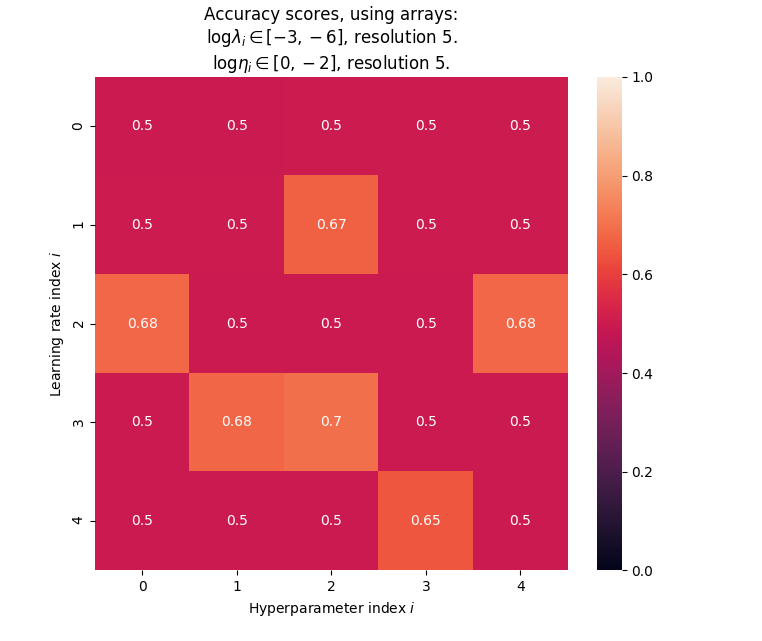
\includegraphics[width=0.4\textwidth]{figures/Ngrid3_acc.png}
%            \caption{Grid search with label $N3$ results. This figure illustrates the accuracy scores for several neural networks with various hyperparameters $\lambda$ and learning rates $\eta$. The range and resolutions of the parameters are in the title, while the indices of the axes range from largest to smallest.}
%            \label{fig:ANNREG1}
%        \end{figure}
%        Figure \ref{fig:ANNREG2} illustrates the area under the cumulative gain curve for network $N3$:
%        \begin{figure}[H]
%            \centering
%            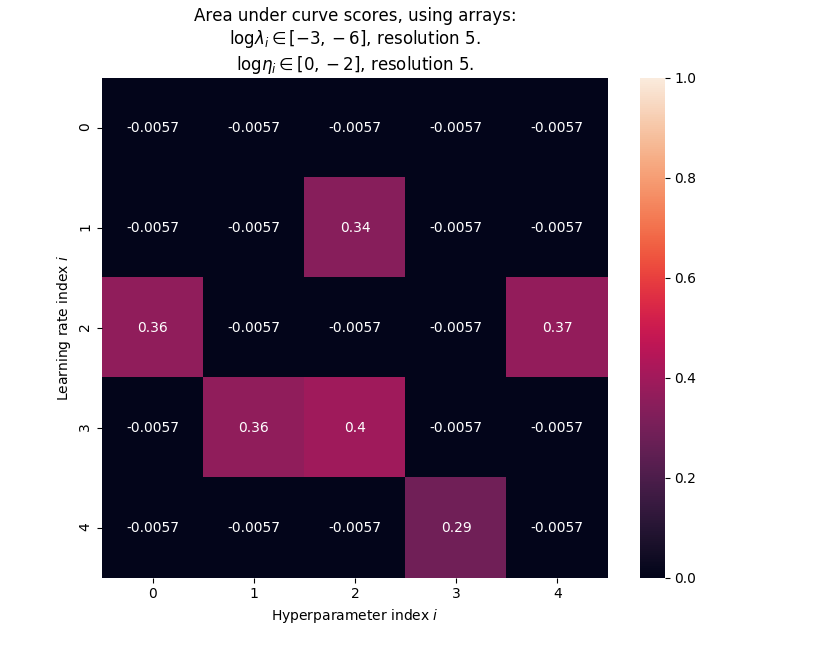
\includegraphics[width=0.4\textwidth]{figures/Ngrid3_auc.png}
%            \caption{Grid search with label $N3$ results. This figure illustrates the area under the cumulative gain curve for several neural networks with various hyperparameters $\lambda$ and learning rates $\eta$. The range and resolutions of the parameters are in the title, while the indices of the axes range from largest to smallest.}
%            \label{fig:ANNREG2}
%        \end{figure}
%        Figure \ref{fig:ANNREG3} illustrates the $F1$ scores for network $N3$:
%        \begin{figure}[H]
%            \centering
%            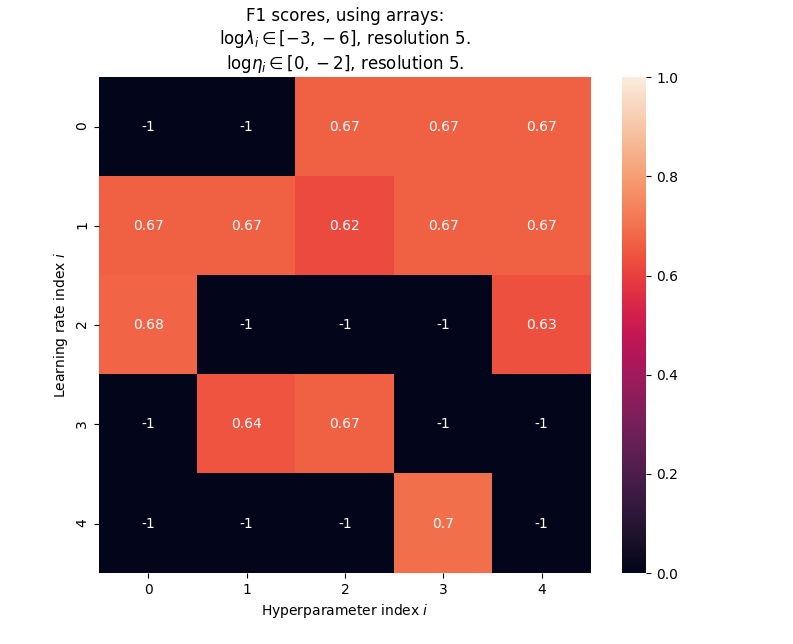
\includegraphics[width=0.4\textwidth]{figures/Ngrid3_F1.png}
%            \caption{Grid search with label $N3$ results. This figure illustrates the $F1$ for several neural networks with various hyperparameters $\lambda$ and learning rates $\eta$. The range and resolutions of the parameters are in the title, while the indices of the axes range from largest to smallest.}
%            \label{fig:ANNREG3}
%        \end{figure}

		The accurary score, F1-score, AUC-score and the gains-ratio of the classification neural network after studing the credit card data can be seen in figure \ref{fig:cc_acc}, \ref{fig:cc_F1}, \ref{fig:cc_auc} and \ref{fig:cc_gr} respectively.

		\begin{figure}[H]
			\centering
			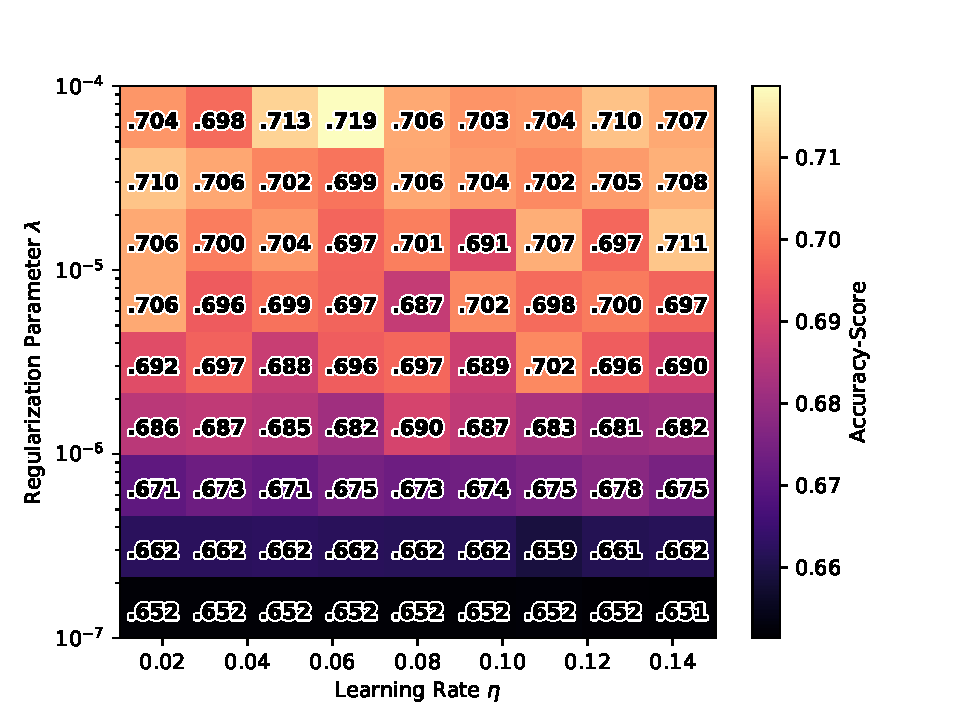
\includegraphics[width=0.5\textwidth]{figures/cc_res_0.pdf}
			\caption{The accurary score of the classification neural network for different $\eta$ and $\lambda$-values after studing the credit card data.}
			\label{fig:cc_acc}
		\end{figure}
		\begin{figure}[H]
			\centering
			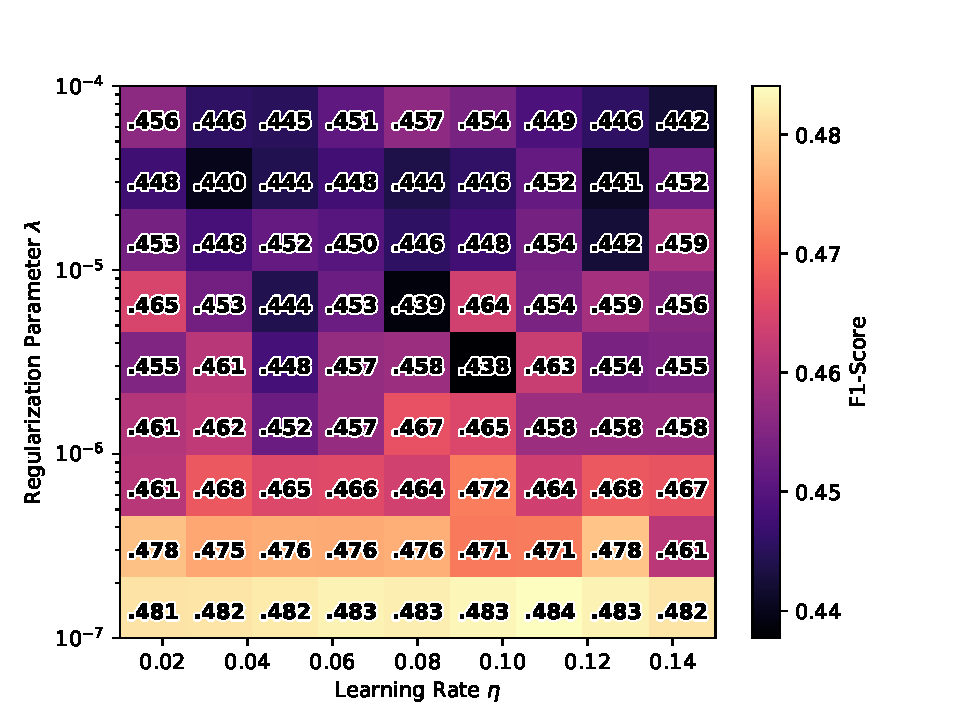
\includegraphics[width=0.5\textwidth]{figures/cc_res_1.pdf}
			\caption{The F1-score of the classification neural network after studing the credit card data.}
			\label{fig:cc_F1}
		\end{figure}
		\begin{figure}[H]
			\centering
			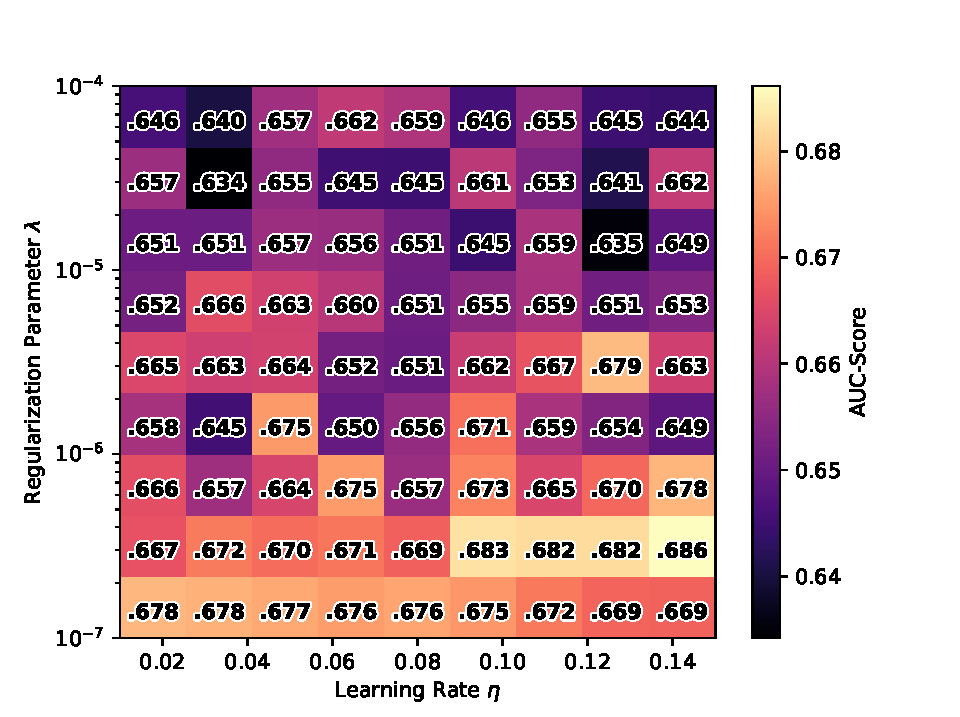
\includegraphics[width=0.5\textwidth]{figures/cc_res_2.pdf}
			\caption{The AUC-score of the classification neural network after studing the credit card data.}
			\label{fig:cc_auc}
		\end{figure}
		\begin{figure}[H]
			\centering
			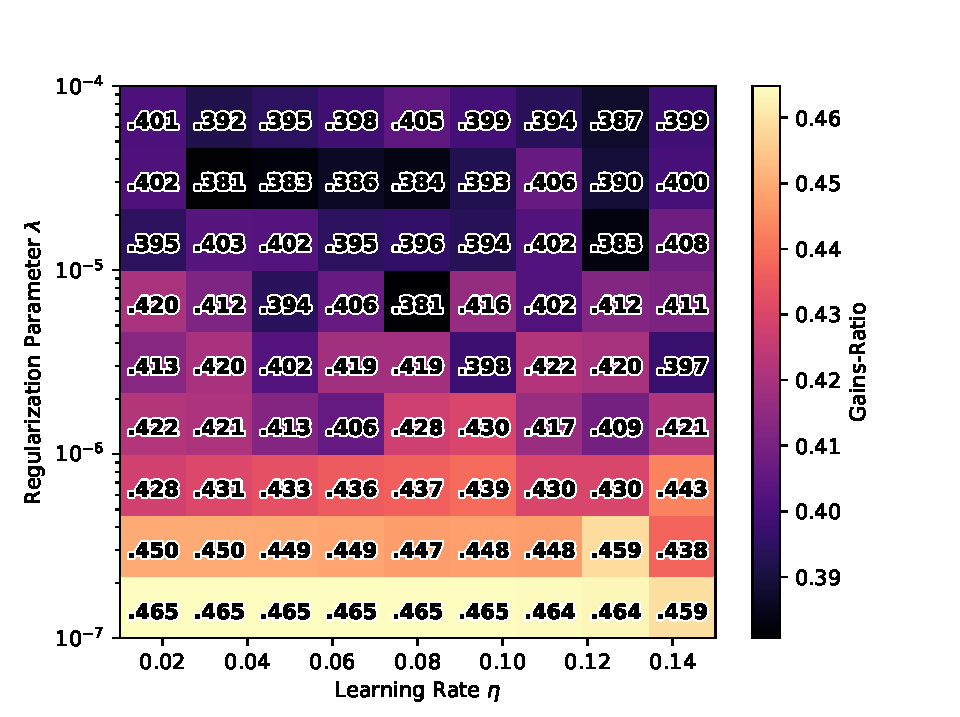
\includegraphics[width=0.5\textwidth]{figures/cc_res_3.pdf}
			\caption{The Gains-Ratio of the classification neural network after studing the credit card data.}
			\label{fig:cc_gr}
		\end{figure}
	
        
        
    \subsection{Regression}
    
    	The mean squared error and the $R^2$-score of the regression neural network after studing Franke's function can be seen in figure \ref{fig:ff_mse} and \ref{fig:ff_r2} respectively.
    
    	\begin{figure}[H]
    		\centering
    		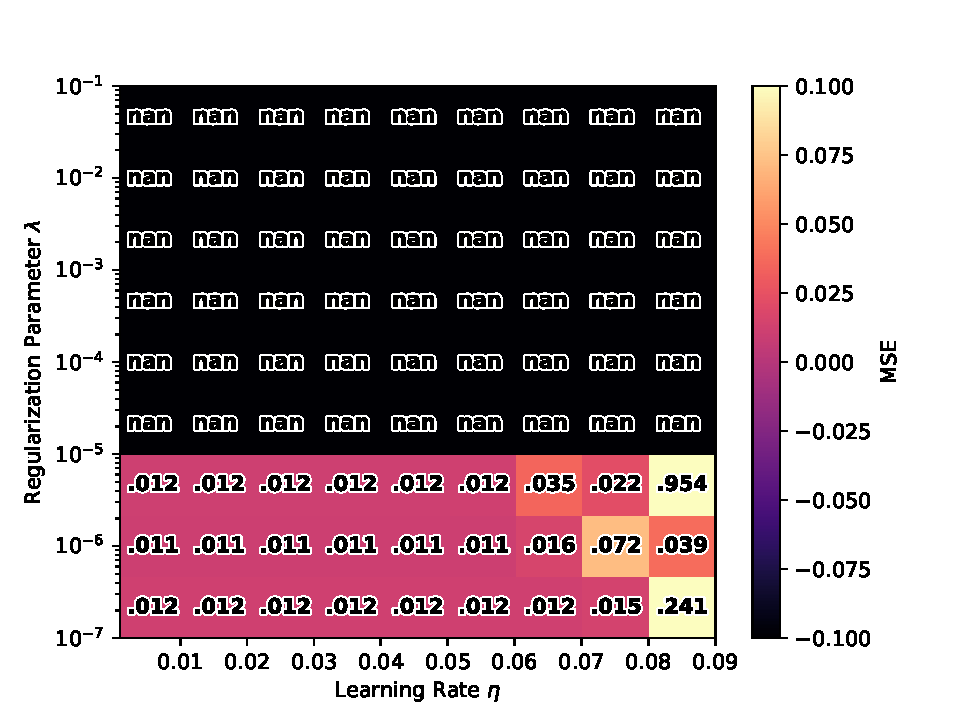
\includegraphics[width=0.5\textwidth]{figures/ff_res_0.pdf}
    		\caption{The mean squared error of the regression neural network after studing Franke's function.}
    		\label{fig:ff_mse}
    	\end{figure}
    	\begin{figure}[H]
    		\centering
    		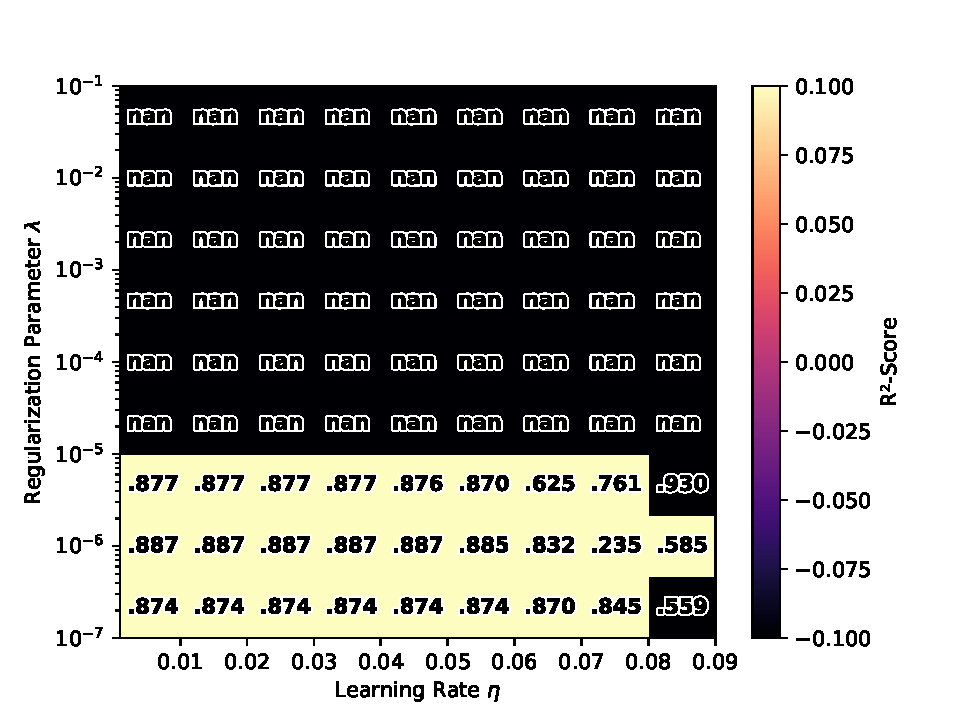
\includegraphics[width=0.5\textwidth]{figures/ff_res_1.pdf}
    		\caption{The $R^2$-score of the regression neural network after studing Franke's function.}
    		\label{fig:ff_r2}
    	\end{figure}
    
    
    	
%        Following is a table from project 1, listing the precision of three regression schemes applied to Franke's function:
%        \begin{table}[H]
%            \centering
%            \caption{Table listing the final results and comparisons of the regressional methods applied to Franke's function with $n=10,000$ data points.}
%            \begin{tabular}[t]{l@{\hskip 0.3in}c@{\hskip 0.3in}c@{\hskip 0.2in}c}
%                \toprule
%                Scheme & MSE minimum & $p_{deg}$ & $\log(\lambda)$ \\
%                \midrule
%                OLS & 0.2493 & 8 & $-$\\
%                Ridge & 0.2489 & 11 & -9\\
%                Lasso & 0.2524 & 8 & -12\\
%                \bottomrule
%            \end{tabular}
%            \label{tab:conclusion_table_Frankes}
%        \end{table}
%        
%        
%        \begin{figure}[H]
%            \centering
%            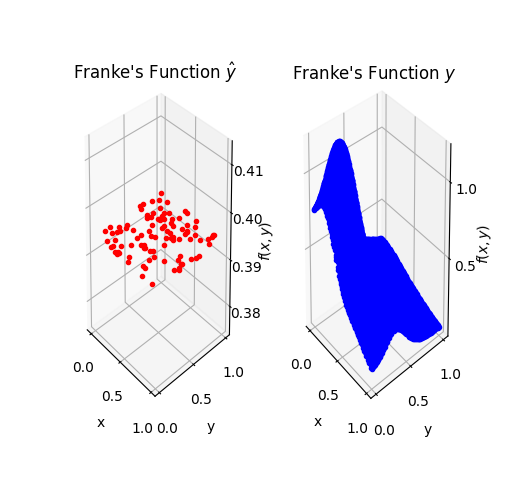
\includegraphics[width=0.4\textwidth]{figures/regression_NNW.png}
%            \caption{The ANN regression on Franke's function. With $MSE=4.08$.}
%            \label{fig:ANNREG}
%        \end{figure}
        
        
        % Table with the least MSE from the two methods
        % (Figure with analysis of regularization parameters and learning rates): this is not specifically asked for in the problem set, it wants: a discussion of reg. params./learning rates
	
	\section{Discussion}
    \subsection{Classification}
        % Logistic regression:
             % Choice of cost-function
             % accuracy: bad/good?
             
        % Neural network
            % Choice of cost-function
            % Optimal weights and biases
            % best reg. params, learning rates
            % accuracy: bad/good?
            
        % COMPARE the two methods: 
            % Give a critical discussion of the results obtained with LR and NN. 
            % Make an analysis of the regularization parameters and learning rates employed to find the optimal accuracy score.
            % Compare choice of cost-functions for the two: did we choose different ones?
        
        % Were the results from Yeh2009 reproduced? 
            % New remarks? 
            % Differences? 
            % Further analysis?
            
    \subsection{Regression}
        Ridge regression accomplished $MSE_{min}=0.2489$ at polynomial degree $p_{deg}=11$ and hyperparameter $\log\lambda=-9$.
        % Linear regression:
             % Choice of cost-function
             
        % Neural network
            % Choice of cost-function
            % Optimal weights and biases
            % best reg. params, learning rates
            
        % COMPARE the two methods: 
            % Give a critical discussion of the results obtained with LR and NN. 
            % Make an analysis of the regularization parameters and learning rates employed to find the optimal accuracy score.
            % Compare choice of cost-functions for the two: did we choose different ones?
     
    \subsection{Comparison of the Methods}
        % Summarize the various algorithms and include a critical evaluation of their pros and cons. Which algorithm is best for the regression and which is best for the classification.
        
        
        
        
        
        % May have been a good idea to add custom weight and bias initialization for each layer added? Would have solved the input mess.
        % There are several factors of the study which could have been performed better; some of which include data preprocessing, grid search rather than ..., and stochasticity between epochs.
        % F1 score is 'ill defined' if the network declares all values to be zeros
        % Should have maybe implemented MPI4PY (code parallelization), and
        % Should have maybe performed some cross validation to find the optimal parameters. This would however have been very computationally inefficient.
	
	\section{Conclusion}
	The multilayered perceptron was found to outperform the stochastic gradient descent algorithm in predicting the credit card data. The optimal accuracy of the SGD algorithm was found to be $61.2\%$ using the l2 regularization parameter $\lambda=10^{-6}$ and a learning rate of at most $\eta=0.06$. This was contrasted by the performance of the neural network which accomplished an accuracy of $71.9\%$ using the l2 regularization parameter $\lambda=10^{-4}$ and learning rate $\eta=0.056$. The ANN was not found to outperform the Ridge scheme at reproducing Franke's function. The Ridge regression produced a minimum of $2\times 10^{-4}$, while the neural network produced a minimum of $0.2$ at best.\\\\
  	Further improvements of the artificial neural network can be made by adding functionalities such as the \textit{dropout rate}, something which has been shown to decrease the variance of the prediction. An improvement can also be made in the grid search methods conducted. Cross validation methods can also be implemented for the search of the optimal parameters. A continuation of the project with improved functionality and greater depth of the research has great potential. This is due to the fact that there are so many factors of the study which can have entire research projects of their own.
  	
	
	\newpage
	

	\onecolumngrid
	\section*{References}
	\bibliography{ref}
	
	\newpage 
	\twocolumngrid
	\fancyhead[L]{Appendices}
	\section*{Appendix A:\\OLS Predictor Derivation}
    Setting the Residual Sum of Squares (RSS) partial derivative with respect to the predictor $\beta$ equal zero yields:
    \begin{equation}
        \pdv{}{\beta}\ RSS = 0
    \end{equation}
    Inserting the expression for RSS (given by $2n\cdot MSE$, where MSE is defined in equation \ref{eq:MSE}) yields:
    \begin{equation}
        \pdv{}{\beta}\ \left( y - X \beta \right)^2 = 0,
    \end{equation}
    rewriting as:
    \begin{equation}
        \pdv{}{\beta}\left( \left( y - X \beta \right)^T\left( y - X \beta \right)\right) = 0,
    \end{equation}
    expanding:
    \begin{equation}
        \pdv{}{\beta}\left( y^Ty - y^TX\beta - \left( X\beta \right)^Ty + \left( X\beta \right)^T\left( X\beta \right) \right) = 0,
    \end{equation}
    removing the factors which are independent of $\beta$ and utilizing the rule
    \begin{equation}
        \left( A^TB \right)^T = B^TA
    \end{equation}
    yields:
    \begin{equation}\label{eq:appA_beta-rel}
        \pdv{}{\beta}\left(- y^TX\beta - \beta^TX^T y + \beta^TX^TX\beta \right) = 0,
    \end{equation}
    Also, seeing as the product $y^TX\beta$ is a scalar, we have that:
    \begin{equation}
        y^TX\beta = \left( y^TX\beta \right)^T = \beta^TX^Ty
    \end{equation}
    Since the transposed of a scalar equals the scalar. This allows us to rewrite equation \ref{eq:appA_beta-rel} to
    \begin{equation}
        \pdv{}{\beta}\left(- 2 \beta^TX^T y + \beta^TX^TX\beta \right) = 0,
    \end{equation}
    Differentiating with respect to $\beta$ yields:
    \begin{equation}
        -2 X^Ty + \pdv{}{\beta} \left( \beta^TX^TX\beta \right) = 0
    \end{equation}
    One more matrix-vector differentiation formula is needed for the final product:
    \begin{align}
        \pdv{(a^TAa)}{a} = 2Aa = 2a^TA
    \end{align}
    for vectors $a$ and a symmetric matrix $A$. We can now derive the final formula for $\beta$:
    \begin{align}
        -2 X^Ty + \pdv{}{\beta} \left( \beta^TX^TX\beta \right) &= 0 \\
        -2 X^Ty + \pdv{}{\beta} \left( \beta^TA\beta \right) &= 0 \\
        -2 X^Ty + 2A\beta &= 0 \\
        -2 X^Ty + 2X^TX\beta &= 0 \\
        -X^Ty + X^TX\beta &= 0
    \end{align}
    by the declaration of $X^TX=A$ being symmetric. This finally yields:
    \begin{align}
        X^TX\beta &= X^Ty \\
        \beta &= \left( X^TX \right)^{-1}X^Ty.
    \end{align}
    \\
    
	\input{sections/appendix-B}
	
\end{document}